\documentclass[%
  a4paper,%    Sets the size of the main font in the document
  titlepage,%  Specifies that a new page should be started after the document title (can be omitted for the `report` class)
  11pt%        Sets the size of the main font in the document
]{article}%    Standard and arguably the most versatile document class. Has `\section` as the top sectioning level

% Sets up the preamble. Please see these .TEX files for details
%%% PREAMBLE :: Encoding and Languages
%
% Sets the proper encoding (UTF-8) for writing in English and Russian


%% Imports required packages
% Sets the font encoding (Latin, Cyrillic)
\usepackage[%
    % T1,%  Latin characters including the accented ones. Suggested for writing papers in English
    T2A%  Cyrillic characters, as well as the Latin ones (first 128 mappings of `T2A` are identical to `T1`). Required for writting papers in Russian
]{fontenc}

% Makes LaTeX interpret text as UTF-8 rather than ASCII
\usepackage[utf8]{inputenc} 

% Enables special symbols and hyphenation for Russian (primary) and English
\usepackage[english,russian]{babel}
%   Encoding and Languages
%%% PREAMBLE :: Graphics
%
% Sets up everything for creating, importing and working with various graphics in the document


%% Imports required packages
% Allows to import, create and manipulate graphics
% \usepackage{graphics}

% Extends the `graphics` package. Allows optional arguments according to the "key=value" scheme. Highly recommended over the `graphics` package
\usepackage{graphicx}

% Provides the tools necessary to create graphic elements (plots, graphs, diagrams) in LaTeX itself
\usepackage{tikz}


%% Sets up paths to the assets
% [graphicx] Points to the folders to search images in.
\graphicspath{%
    {././img/}%  Assuming this file is in the root's "preamble/" folder, it points to the root's "img/" folder
}

%% Sets up required TikZ libraries
% [tikz] Allows for more precise coordinate calculations
\usetikzlibrary{calc}
% [tikz] Enables varios markings at any place of a line
\usetikzlibrary{decorations.markings}
%   Graphics paths and parameters
%%% PREAMBLE :: Layout
%
% Sets the general layout of the document (margins, spacing, title format, section format, headers, footers, referencing style, etc.)


%% Imports required packages
% Provides more granular control over the layout of `enumerate', `itemize' and `description'
\usepackage[shortlabels]{enumitem}

% Sets the pages' headers and footers for the main part of the document
\usepackage{fancyhdr}

% Sets the pages' layout
\usepackage[%
    a4paper,%         Same as the size of the article
    hmargin=3.175cm,% Equivalent to `left=3.175cm, right=3.175cm`
    vmargin=2.54cm%   Equivalent to `top=2.54cm, bottom=2.54cm`
]{geometry}

% Provides extensive handling and customization of cross-referencing and creating hypertext links
\usepackage[%
    pdfusetitle%  Catches the document's @title and @author arguments for \hypersetup 
]{hyperref}

% Enables conditional commands like `\ifthenelse` and `\whiledo` 
\usepackage{ifthen}

% Indents first paragraph after (sub)section headers
\usepackage{indentfirst}

% Allows reference to the document's last page's number (required for the fancyhdr footer) 
\usepackage{lastpage}

% Sets up easily configurable ragged text environment (required for the `lecture` environment to display the headers and footers properly)
\usepackage{ragged2e}

% Edits the layout of sections, subsections, etc.
\usepackage[%
    compact,% Reduces the spacing above and below the titles
    sc,%      Sets the default font shape to `scientific`
    center%   Aligns to the center of a page
]{titlesec}

% Provides an underline command which breaks over line ends. Imported for underling URLs (see the `\myurl` command)
\usepackage[%
    normalem% Disables redefining of `\em` and `\emph`
]{ulem}


%% Sets up general indentation
\setlength{\parindent}{2.3em}%         Paragraph indentation
%\setlength{\parskip}{0.2cm}%           Spacing between paragraphs
%\renewcommand{\baselinestretch}{1.4}%  Line spacing


%% Handles with overfulls and page breaks
% Changes the setting of paragraphs that would have produced over-full boxes, tries an extra pass with pretending that every line has an additional bit of space. Prevents the overall badness exceeding 1000
\setlength{\emergencystretch}{1.5em}
\clubpenalty=10000   % Prohibits page-breakings after just one paragraph line
\widowpenalty=10000  % Prohibits page-breakings after last paragraph lines


%% Sets up the lists
% [enumitem] Defines the `statesp` and `casesp` lists 
\newlist{statesp}{enumerate}{1}
\newlist{casesp}{enumerate}{2}

% [enumitem] Makes the `enumerate` list more compact
\setenumerate{%
    nosep,%            Removes vertical spacing
    nolistsep,%        Removes spacing between the list itself and the neighbouring paragraphs
    noitemsep,%        Removes spacing between items and paragraphs
    topsep=0pt,%       Removes spacing between first item and preceding paragraph
    parsep=0pt,%       Removes spacing between paragraphs within an item
    partopsep=0pt,%    Removes extra spacing added to `\topsep`
    label=(\arabic*)%  Sets the default label
}

% [enumitem] Makes the `itemize` list more compact
% Sets the default label for the first level
\renewcommand{\labelitemi}{$\Diamond$}
\setlist[itemize]{%
    nosep,%                 Removes vertical spacing
    nolistsep,%             Removes spacing between the list itself and the neighbouring paragraphs
    noitemsep,%             Removes spacing between items and paragraphs
    topsep=0pt,%            Removes spacing between first item and preceding paragraph
    parsep=0pt,%            Removes spacing between paragraphs within an item
    partopsep=0pt,%         Removes extra spacing added to `\topsep`
}

% [enumitem] Sets the `statesp` list
\setlist[statesp]{%
    align=left,%                Aligns the labels properly
    nosep,%                     Removes vertical spacing
    nolistsep,%                 Removes spacing between the list itself and the neighbouring paragraphs
    noitemsep,%                 Removes spacing between items and paragraphs
    topsep=0pt,%                Removes spacing between first item and preceding paragraph
    parsep=0pt,%                Removes spacing between paragraphs within an item
    partopsep=0pt,%             Removes extra spacing added to `\topsep`
    font=\normalfont\bfseries%  Boldens the labels
}
\setlist[statesp,1]{%
  label=Пункт~(\arabic*):,%     Sets label format for the top level
  ref=\arabic*%                 Sets cross-ereferencing format for the top level
}

% [enumitem] Sets the `casesp` list
\setlist[casesp]{%
    align=left,%
    nosep,%
    noitemsep,%
    parsep=0pt,%
    partopsep=0pt,%
    font=\normalfont\bfseries%
}
\setlist[casesp,1]{%
    label=Случай~\arabic*:,%
    ref=\arabic*%
}
\setlist[casesp,2]{%
    label=Случай~\thecasespi.\roman*:,%
    ref=\thecasespi.\roman*%
}


%% [fancyhdr, ifthen, lastpage] Sets up the header and footer parts of pages' layout
% Clears header and footer completely
\fancyhf{}
% Puts the current subsection number and name on the left side of the header
% If subsection has been reset by a new section it puts the current section number and name instead
% The `\leftmark` command outputs the number and name of the current section in the `article` document class, while the `\rightmark` does it for current subsection
\lhead{
    \scshape\small\ifthenelse{%
        \equal{\rightmark}{}}%
        {\bfseries\nouppercase{\leftmark}}%
        {\S\rightmark}
}
% Puts the current lecture number on the right side of the header
\rhead{
    \it{Лекция~\textnumero\themylecture}
}
% Puts the pae counter on the right side of the footer
\rfoot{
    Стр. \thepage~/ \pageref*{LastPage}
}
% Tweaks the width of the top rule
\renewcommand{\headrulewidth}{0.1pt}
% Adjusts the topmargin for fancyhdr
\setlength{\headheight}{14pt}
% Defines an alternative page style for the sections' supplementary material
\fancypagestyle{supplementary}{%
    \lhead{
        \scshape\small\bfseries\nouppercase{\leftmark}
    }
}


%% Sets up the linking style and the PDF-specific options
% [hyperref] Overrides the `\and` command while creating the document's metadata (in case of several authors)
\pdfstringdefDisableCommands{\def\and{и}}
% [hyperref] Sets up links' style and metadata information
\makeatletter%  Changes the `@` symbol's category from `other` (catcode: 12) to `letter` (catcode: 11), so it's treated as a normal letter
\DeclareUrlCommand\myurl@@{%
    \def\UrlFont{\color{blue}}%
    \def\UrlLeft{\uline\bgroup}%
    \def\UrlRight{\egroup}
}
\def\myurl@#1#2{\hyper@linkurl{\myurl@@{#2}}{#1}}
\DeclareRobustCommand*\myurl{\myurl@}
\hypersetup{%
    linktocpage=true,%        Makes the page numbers from the Table Of Contents interactive
    colorlinks=true,%         Colours the (cross-referencing) links
    urlcolor=blue,%           Sets the colour of URLs
    bookmarksopen=true,%      Makes the bookmark bar open by default in a PDF reader
    pdfpagemode=FullScreen,%  Makes a PDF reader open the document in full screen
    pdfauthor={\@author},%    Sets the document's author(s) based upon the `\author`
    pdftitle={\@title}%       Sets the document's title based upon the `\title`
}
\makeatother%  Changes the `@` symbol's category from `letter` (catcode: 11) to `other` (catcode: 12), so it could be safely used in macros


%% [titlesec] Sets up the format of sections and subsections
% Converts the sections' labels to the Roman numerals
\renewcommand{\thesection}{\Roman{section}}
\titleformat%
    {\section}%                           Redefines the sectioning command (`\section`)
    [block]%                              Sets paragraph's shape so a section's label and title are on the same line
    {\centering\Large\scshape\bfseries}%  Sets label's and title's format
    {\thesection.}%                       Sets label
    {0.3cm}%                              Sets the spacing between label and title body
    {}%                                   Sets the after-code
\titleformat%
    {\subsection}%
    [block]%
    {\centering\large\scshape}%
    {\S\thesubsection.}%
    {0.3cm}%
    {}
% Adjusts the vertical spacing for the sections' titles
\titlespacing*%
    {\section}%   Sets spacing around the sections' titles
    {0cm}%        Sets the left margin
    {1cm}%        Sets the vertical space before the title
    {0.5cm}%      Sets the vertical space after the title
\titlespacing*%
    {\subsection}%
    {0cm}%
    {0.4cm}%
    {0.2cm}
% Starts each section (except the first one) on a new page
% N.B.: Depends on the definition of `\thesection` above
\newcommand{\sectionbreak}{
    \ifthenelse{%
        \equal{\thesection}{I}}%  If section's number is "I"
        {}%                       Skip
        {\clearpage}%             Else start the section on a new page
}


%% [hyperref, ragged2e] Defines an environment that sets up the lectures' header and footer. Takes one mandatory argument -- the lecture's date -- and one optional argument -- the lecture's number. If the optional argument is passed, it updates a counter
% Initializes a counter for lecture numbers
\newcounter{mylecture}
\newenvironment{lecture}[2][\themylecture]%
    {%
        % If the optional argument isn't passed, increment the default counter
        \refstepcounter{mylecture}
        \vspace{0.15cm}
        % Since arguments passed to an environment are only available for the start-code, a hack with storing these arguments is used
        % Defines the lecture's number as the optional argument if it's been passed, or as the default counter's value otherwise. `\def` is used to overwrite the commands each time
        \def\lecnum{#1}
        \def\lecdate{#2}

        \raggedleft{
            \scriptsize
            \textit{Лекция \textnumero\lecnum~от \lecdate}
            \label{lec:no#1}
        }
        \hrule
        \vspace{0.3cm}
        \justify
    }%
    {%
        % Updates the counter, so the next lecture's number agrees.
        \setcounter{mylecture}{\lecnum}
        \vspace{0.3cm}
        \hrule
        \raggedright{
            \scriptsize
            \textit{\hyperref[lec:no\lecnum]{Вернуться} к началу Лекции \textnumero\lecnum.}
        }
        \justify
    }
%     General layout
%%% PREAMBLE :: Mathematical packages
%
% Loads a set of packages developed for the American Mathematical Society
% Sets up theorem environments and additional commands/operators
% Essential for compiling any mathematical research paper


%% Imports required packages
% Provides enhancements for properly outputing mathematical formulas
\usepackage{amsmath}

% Internally loads the `amsfonts` package, provides an extended symbol collection
\usepackage{amssymb}

% Provides support of various environments (Theorem, Lemma, proof, etc.)
\usepackage{amsthm}

% Enables support of commutative diagrams
% \usepackage{amscd}

% Enables support of blackboard bold letters, Fraktur letters and miscellaneous symbols
% \usepackage{amsfonts}


%% Defines various maths environments (Theorem, Lemma, proof, etc.). Both numbered and unnumbered
% [amsthm] Defines the Theorem-style environments
\theoremstyle{plain}
\newtheorem{ntheorem}{Теорема}[section]
\newtheorem{nlemma}{Лемма}[section]
\newtheorem{nproposition}{Предложение}[section]
\newtheorem{ncorollary}{Следствие}[section]
\newtheorem*{theorem}{Теорема}
\newtheorem*{lemma}{Лемма}
\newtheorem*{proposition}{Предложение}
\newtheorem*{corollary}{Следствие}
\newtheorem*{hypothesis}{Гипотеза}
\newtheorem*{test}{Признак}

% [amsthm] Defines the Definition-style environments
\theoremstyle{definition}
\newtheorem{ndefinition}{Определение}[section]
\newtheorem{nstatement}{Утверждение}[section]
\newtheorem{nexample}{Пример}[section]
\newtheorem*{definition}{Определение}
\newtheorem*{statement}{Утверждение}
\newtheorem*{example}{Пример}

% [amsthm] Defines the Remark-style environments
\theoremstyle{remark}
\newtheorem{nproblem}{Задача}[section]
\newtheorem{nremark}{Замечание}[section]
\newtheorem*{problem}{Задача}
\newtheorem*{remark}{Замечание}

% [amsthm, amssymb] Redefines the proof's QED symbol
\renewcommand{\qedsymbol}{$\blacksquare$}

% [amsthm, amssymb] Defines the `Solution` environment
\newenvironment{solution}
    {%
        \renewcommand{\qedsymbol}{$\square$}%
        \begin{proof}[Решение]%
    }
    {\end{proof}}


%% Defines and redefines common mathematical operators
% [amsfonts] Defines commonly used sets (fields)
\newcommand{\field}[1]{\ensuremath{\mathbb{#1}}}
\newcommand{\CC}{\field{C}}    % Complex numbers
\renewcommand{\AA}{\field{A}}  % Algebraic numbers
\newcommand{\RR}{\field{R}}    % Real numbers
\newcommand{\QQ}{\field{Q}}    % Rational numbers
\newcommand{\ZZ}{\field{Z}}    % Integer numbers
\newcommand{\NN}{\field{N}}    % Natural numbers
\newcommand{\EE}{\field{E}}    % Field extension (see IV.3)

% [amsfonts] Defines commonly used notation for rings
\newcommand{\ring}[1]{\ensuremath{\mathcal{#1}}}
\newcommand{\rr}{\ring{R}}

% [amsmath] Changes `\Re` and `\Im` from Fraktur to Roman and puts its argument in parentheses
\renewcommand{\Re}[1]{\operatorname{Re}\left( #1 \right)}
\renewcommand{\Im}[1]{\operatorname{Im}\left( #1 \right)}

% [amsmath] Redefines the predefined operators of AMSMATH to Russian notation and puts its argument in parentheses (e.g. sin x => sin(x), tan x => tg(x), etc.)
% If any default operators are needed, the corresponding lines can be commented out
% Trigonometric functions
\renewcommand{\sin}[1]{\operatorname{sin}\left( #1 \right)}
\renewcommand{\cos}[1]{\operatorname{cos}\left( #1 \right)}
\renewcommand{\tan}[1]{\operatorname{tg}\left( #1 \right)}
\renewcommand{\cot}[1]{\operatorname{ctg}\left( #1 \right)}
\renewcommand{\arcsin}[1]{\operatorname{arcsin}\left( #1 \right)}
\renewcommand{\arccos}[1]{\operatorname{arccos}\left( #1 \right)}
\renewcommand{\arctan}[1]{\operatorname{arctg}\left( #1 \right)}
\renewcommand{\sec}[1]{\operatorname{sec}\left( #1 \right)}
\renewcommand{\csc}[1]{\operatorname{cosec}\left( #1 \right)}
\renewcommand{\sinh}[1]{\operatorname{sh}\left( #1 \right)}
\renewcommand{\cosh}[1]{\operatorname{ch}\left( #1 \right)}
\renewcommand{\tanh}[1]{\operatorname{th}\left( #1 \right)}
\renewcommand{\coth}[1]{\operatorname{cth}\left( #1 \right)}
% Logarithms
\renewcommand{\log}[1]{\operatorname{log}\left( #1 \right)}
\renewcommand{\ln}[1]{\operatorname{ln}\left( #1 \right)}
\renewcommand{\lg}[1]{\operatorname{lg}\left( #1 \right)}
% Limits
\renewcommand*{\limsup}{\varlimsup}
\renewcommand*{\liminf}{\varliminf}
% Defines a limit operator with both upper and lower bars
\DeclareMathOperator*{\limsi}{\overline{\underline{lim}}}
\newcommand*{\limsupinf}[1]{\limsi\left( #1 \right)}
% Miscellaneous
\renewcommand{\deg}[1]{\operatorname{deg}\left( #1 \right)}
\renewcommand{\det}[1]{\operatorname{det}\left( #1 \right)}
\renewcommand{\dim}[1]{\operatorname{dim}\left( #1 \right)}
\renewcommand{\exp}[1]{\operatorname{exp}\left( #1 \right)}
\renewcommand{\gcd}[1]{\textrm{НОД}\left( #1 \right)}
\renewcommand{\hom}[1]{\operatorname{Hom}\left( #1 \right)}
\renewcommand{\ker}[1]{\operatorname{Ker}\left( #1 \right)}

% [amssymb] Redefines the `greater than` and `less than` signs
\renewcommand{\ge}{\geqslant}
\renewcommand{\le}{\leqslant}

% Redefines the look of some Greek letters commonly used as variables or functions
\renewcommand{\epsilon}{\varepsilon}
\renewcommand{\phi}{\varphi}

% Redefines the universal and existential quantifiers to adjust spacing
\let\oldforall\forall
\let\oldexist\exists
\renewcommand{\forall}{\oldforall \, }
\renewcommand{\exists}{\oldexist \: }
\newcommand\existu{\oldexist! \: }


%% Defines additional commands for document-specific notations
% Defines the `divisible by` symbol (three vertical dots with the right spacing)
\DeclareRobustCommand{\divisibleby}{%
    \mathrel{%
        \text{%
            \vbox{%
                \baselineskip.65ex%
                \lineskiplimit0pt%
                \hbox{.}\hbox{.}\hbox{.}%
            }%
        }%
    }%
}
% Provides flexible vertical bars for `\abs`
% It measures how much larger the content is allowed to get before the delimiters start growing, but by setting it to a negative value delimiters always grow
\delimitershortfall-1sp
\newcommand{\abs}[1]{\ensuremath{\left| #1 \right|}}
\newcommand{\lcd}[1]{\textrm{НОК}\left( #1 \right)}
\newcommand{\congr}[3]{\ensuremath{#1 \equiv #2 \pmod #3}}
\newcommand{\notcongr}[3]{\ensuremath{#1 \not\equiv #2 \pmod{#3}}}
\newcommand{\sfrac}[2]{\ensuremath{#1 / #2}}
\newcommand{\divides}{\mid}
\newcommand{\notdivides}{\nmid}
\newcommand{\divby}{\divisibleby}
\newcommand{\notdivby}{\not\divby}
\newcommand{\1}{\textbf{1}}
\DeclareMathOperator*{\Res}{Res}
\newcommand{\bigO}[1]{\ensuremath{\mathcal{O}\left( #1 \right)}}


%% Toggles the display style to be equation-like everywhere
% It's generally not recommended, as it increases the spacing between the lines and tears the standard baseline. But in our case it improves the document's readability
\everymath{\displaystyle}
%      Mathematical packages, theorem environments and additional commands/operators


% Sets up the .PDF's metadata (see preamble/layout.tex)
\title{Конспект лекций по Теории Чисел}
\author{Артемий Соколов \and~Артемий Геворков}


\begin{document}
    % Makes the titlepage's layout wider
\newgeometry{
    hmargin=3.5cm,% Equivalent to `left=3.5cm, right=3.5cm`
    vmargin=1.7cm%  Equivalent to `top=1.7cm, bottom=1.7cm`
}


\begin{titlepage}
    % Sets the page numbering style to Roman uppercase, removing the ambiguity for hyperref
    % Since it's the titlepage, it'll only show up in a PDF viewer
    \pagenumbering{Roman}

    \centering

    \large
    \scshape
    МОСКОВСКИЙ ГОСУДАРСТВЕННЫЙ УНИВЕРСИТЕТ~\\
    имени М.В. ЛОМОНОСОВА
 
    \vspace{0.8cm}
 
    МЕХАНИКО--МАТЕМАТИЧЕСКИЙ ФАКУЛЬТЕТ
    
    \vfill
    
    % Sets the vector logo of Mechmath MSU, see the .tikz file for details
    % Renders the vector-graphic logo of Mechmath MSU
% I decided to make it using the standard TikZ tools only rather than using Bezier curves, because the logo is quite precise
% (also because I'm a badass)
% See the titlepage
%
% One may alter the logo's scale and color using the TikZ options below
\tikz[rounded corners,color=black!92,scale=0.8]{
    % Draws the background 8x8 grid
    \draw[step=1cm] 
        (0, 0) grid (8, 8);

    % Constructs the right strip of the Moebius band
    \filldraw[ultra thick,fill=white]
        (5.04, 7) 
        .. controls(6.5, 5.7) .. (7.12, 4.88)
        .. controls(7.18, 4) and (6.91, 3.3) .. (6.3, 3)
        .. controls(4.6, 6.2) and (4.1, 6.1) .. (3.5, 5.82)
        .. controls(4.1, 6.75) .. (5.04, 7);

    % Constructs the left strip of the Moebius band
    \filldraw[ultra thick,fill=white]
        (5.04, 7) 
        .. controls(4, 6.88) .. (3.1, 6.6)
        .. controls(1.37, 5.25) and (1.08, 4) .. (1.025, 3.05)
        .. controls(1.2, 2.5) .. (2, 2)
        .. controls(3, 4.75) .. (5.04, 7);

    % Constructs the integral shape
    \filldraw[ultra thick]
        (4, 7.89)
        .. controls(4.91, 7.1) and (5.45, 8.43) .. (4.45, 8.52)
        .. controls(3.42, 8.24) and (3.4, 7.41) .. (3.35, 7)
        .. controls(3.4, 6) .. (3.54, 4)
        .. controls(3.81, 2) .. (4.06, 1)
        .. controls(4.2, 0.21) and (4.05, 0.158) .. (4, 0.11)
        .. controls(3.09, 0.7) and (2.65, -0.43) .. (3.64, -0.52)
        .. controls(3.83, -0.48) and (4.32, -0.29) .. (4.5, 0)
        .. controls(4.6, 0.24) and (4.64, 0.7) .. (4.63, 1)
        .. controls(4.47, 2) .. (4.34, 4)
        .. controls(4.1, 5.7) .. (3.84, 7.54)
        .. controls(3.87, 7.82) .. (4, 7.89);

    % Constructs the front strip of the Moebius band
    \filldraw[ultra thick,fill=white]
        (1.025, 3.05)
        .. controls(1.24, 2.6) .. (3.3, 2.42)
        .. controls(4.5, 2.32) and (7, 3.4) .. (7.1, 4.15)
        .. controls(6.72, 2.6) and (7, 1.9) .. (6.1, 1.55)
        .. controls(4.12, 1.05) .. (2.3, 1.02)
        .. controls(1.52, 1.86) and (1.06, 2.7) .. (1.05, 3.05);
}


    \vspace{0.35cm}

    \Huge
    Конспект лекций по~\\
    \textbf{%
        Теории Чисел
    }

    \vspace{0.5cm}

    \large
    Лектор --- 
    \textbf{%
        Герман Олег Николаевич
    }

    \vspace{0.8cm}
    
    7-й семестр, первый поток, осень 2017

    \vspace{1.8cm}

    \normalsize
    Конспект подготовили

    \vspace{0.4cm}

    \begin{minipage}{0.49\textwidth}
        \begin{flushleft}
            \textbf{Соколов Артемий\\(группа 405)}\\
            нечётные лекции
        \end{flushleft}
    \end{minipage}
    \begin{minipage}{0.49\textwidth}
        \begin{flushright}
            \textbf{Геворков Артемий\\(группа 402)}\\
            чётные лекции
        \end{flushright}
    \end{minipage}

    \vspace{1.5cm}

    \vfill
    \textnormal{Москва, 2017 г.}
\end{titlepage}


% Resets the layout to the one defined in preamble/layout.tex for all proceeding pages
\restoregeometry

    % Sets the page numbering style to Roman lowercase, removing the ambiguity for hyperref
\pagenumbering{roman}


\section*{Предисловие}


\itshape

\textbf{Disclaimer!} Это не курс лекций и не методичка, а всего лишь конспект курса, набранный в системе компьютерной вёрстки \LaTeXe~и не претендующий на истину в последней инстанции. Не исключено также, что в данной версии присутствуют неточности и опечатки, хотя мы --- авторы --- и старались свести их количество к минимуму. В любом случае этот документ предлагается использовать на свой страх и риск, и мы не несём ответственности за успешность подготовки по данному материалу, а также за его использование в качестве ``шпоры'' на коллоквиумах или (боже упаси!) экзаменах.

Конспект состоит из 14-ти лекций, прочитанных Олегом Николаевичем Германом --- доцентом кафедры теории чисел мехмата МГУ. Курс был прочитан в 7-ом семестре мехмата осенью 2017 года и состоит из трёх основных частей:
\begin{enumerate}
    \item Асимптотический закон распределения простых чисел:
        % !IMPORTANT!
        % The `\[...\]` syntax should always be used over `$$...$$` when working in LaTeX, as it doesn't screw up the vertical spacing
        \[
            \pi(x) = \sum_{p \le x} 1 \sim \frac{x}{\ln{x}}.
        \]
    \item Теорема Дирихле о простых числах в арифметических прогрессиях: если ${\gcd{l,\, m} = 1}$, то существует бесконечное количество таких простых $p$, что ${\congr{p}{l}{m}}$.
    \item Теоремы о том, что $e$ и $\pi$ — иррациональные и трансцендентные числа.
\end{enumerate}

Этот конспект был подготовлен и за\TeXан студентами Артемием Соколовым, группа 405 (нечётные лекции) и Артемием Геворковым, группа 402 (чётные лекции) ещё в декабре 2017 года. За основу нами был взят конспект Юлии Зайцевой.

В декабре 2020 года я --- Артемий Геворков --- решил вернуться к этому документу, чтобы улучшить качество вёрстки, подправить некоторые неточности и привести сам код в порядок (с учётом всего моего накопленного опыта по вёрстке в системе \LaTeXe~--- оформления конспектов, домашек, курсовых и т.д. --- за все годы обучения на мехмате). Кроме того, я снабдил некоторые доказательства пояснительными рисунками, которые были нарисованы с помощью пакета~\texttt{tikz}. Также я переписал б\'{о}льшую часть кода преамбулы документа, снабдив сам код подробными комментариями. Если кому-то из читателей понравится данная вёрстка, и он или она захочет оформить свой конспект (или любой другой документ) в подобной вёрстке, то, надеюсь, этих комментариев будет достаточно, чтобы разобраться в коде и настроить его под свои нужды.

В перспективе я ещё планирую добавить решения всех упражнений из данного курса лекций, а также решения ряда заданий, разобранных на семинарских занятиях Олега Николаевича.

Данная версия документа была скомпилирована \today~Последняя версия конспекта вместе со всеми его исходными файлами всегда будет доступна в этом~\href{https://github.com/gevartrix/msu-numbertheory-conspect}{Github--репозитории} (ссылка кликабельна). Если вы нашли в самой свежей версии документа какую-нибудь неточность, или если у вас есть какие-либо вопросы/замечания --- пожалуйста, откройте в репозитории issue или присылайте pull request.

Спасибо Юлии Зайцевой, Виталию Лобачевскому, Всеволоду Гусеву, Кириллу Сосову, Сергею Джунусову, Айку Эминяну, Александру Думаревскову и команде Алгебрача за поиск ошибок и помощь в оформлении данного материала.

\normalfont
\newpage

    % Resets the page numbering style, so the main content starts from page 1
    \pagenumbering{arabic}
    \tableofcontents
    % Encapsulates the Table of Contents 
    \newpage

    % Toggles the fancyhdr configuration for the proceeding pages
    \pagestyle{fancy}

    \begin{lecture}{5 сентября 2017 г.}
        \section{Асимптотический закон распределения простых чисел}
\label{sec:I_prime-number-theorem}

\begin{remark}
    Впредь, если мы будем писать сумму вида $\sum_{\dots p \dots} \dots$, то будет подразумеваться, что $p$ --- простое число.
\end{remark}


\subsection{Оценки Чебышёва}
\label{subsec:I-1}

Изучение распределения простых чисел непосредственно связано с изучением следующих функций:
\begin{itemize}
    \item
        $\pi(x) = \sum_{p \le x} 1$ --- количество простых чисел, не превосходящих $x$;
    \item
        $\theta(x) = \sum_{p \le x} \ln{p} = \ln{\prod_{p \le x} p}$ --- $\theta$--функция Чебышёва;
    \item
        $\psi(x) = \sum_{p^\alpha \le x} \ln{p} 
        = \sum_{p \le x} \left[ \dfrac{\ln{x}}{\ln{p}} \right] \ln{p} 
        = \ln{\lcd{1, 2, \dots, \left[ x \right]}}$ --- $\psi$--функция Чебышёва.
\end{itemize}

Как эти функции связаны? Оказывается, что следующим соотношением:
\begin{nlemma}
\label{lm:I-1}
    \[
        \limsupinf{\frac{\theta(x)}{x}}
        = \limsupinf{\frac{\psi(x)}{x}}
        = \limsupinf{\frac{\pi(x)}{\sfrac{x}{\ln{x}}}},
        \qquad x \to \infty.
    \]
\end{nlemma}
\begin{proof}
    Заметим, что
    \[
        \theta(x) \le \psi(x)
        \le \sum_{p \le x} \left[ \frac{\ln{x}}{\ln{p}} \right] \ln{p} 
        = \ln{x} \sum_{p \le x} 1 = \pi(x)\ln{x}.
    \]
    Следовательно, получаем соотношение
    \[
        \limsupinf{\frac{\theta(x)}{x}}
        \le \limsupinf{\frac{\psi(x)}{x}}
        \le \limsupinf{\frac{\pi(x)}{\sfrac{x}{\ln{x}}}}.
    \]
    Для доказательства нам теперь нужны неравенства ``в другую сторону''. Рассмотрим простые числа на отрезке $\left[ x^\alpha,\, x \right]$ для некоторого фиксированного $0 < \alpha < 1$. 
    Тогда
    \begin{align*}
        \theta(x) = \sum_{p \le x} \ln{p} \ge \sum_{x^\alpha < p \le x} \ln{p} &> \ln{x^\alpha} \sum_{x^\alpha < p \le x} 1 \\
        &= \alpha \ln{x}\left( \pi(x) - \pi\left(x^{\alpha}\right) \right).
    \end{align*}
    Разделив полученное выражение на $x$, получаем
    \[
        \frac{\theta(x)}{x} 
        > \alpha\left( \frac{\pi(x)}{\sfrac{x}{\ln{x}}} - \frac{\ln{x}}{x^{1 - \alpha}} \right),
        \qquad \forall\ 0 < \alpha < 1.
    \]
    Так как $\frac{\ln{x}}{x^{1-\alpha}} \to 0$ при $x \to \infty$, то
    \begin{align*}
        \limsup\left( \frac{\theta(x)}{x} \right) &
        \ge \limsup\left( \alpha\frac{\pi(x)}{\sfrac{x}{\ln{x}}} \right) 
        = \alpha \limsup\left( \frac{\pi(x)}{\sfrac{x}{\ln{x}}} \right), \\
        \liminf\left( \frac{\theta(x)}{x} \right) &
        \ge \liminf\left( \alpha\frac{\pi(x)}{\sfrac{x}{\ln{x}}} \right) 
        = \alpha \liminf\left( \frac{\pi(x)}{\sfrac{x}{\ln{x}}} \right).
    \end{align*}
    Эти неравенства выполняются для любых $\alpha \in (0,\, 1)$, поэтому получаем неравенство ``в другую сторону'':
    \[
        \limsupinf{\frac{\theta(x)}{x}}
        \ge \limsupinf{\frac{\pi(x)}{\sfrac{x}{\ln{x}}}}.
    \]
    Таким образом мы получили утверждение Леммы:
    \[
        \limsupinf{\frac{\theta(x)}{x}}
        = \limsupinf{\frac{\psi(x)}{x}}
        = \limsupinf{\frac{\pi(x)}{\sfrac{x}{\ln{x}}}},
        \qquad x \to \infty.
    \]
\end{proof}

\begin{ntheorem}[Оценки Чебышёва]
\label{thm:I-1}
    Существуют $a,b > 0$ такие, что
    \[
        a \frac{x}{\ln{x}} \le \pi(x) \le b \frac{x}{\ln{x}}.
    \]
\end{ntheorem}

Перед доказательством этой теоремы сформулируем и докажем несколько вспомогательных лемм.
\begin{nlemma}
\label{lm:I-2}
    \[
        \prod_{p \le n} p \le 4^n.
    \]
\end{nlemma}
\begin{proof}
    Будем доказывать методом математической индукции по $n$.~\newline
    \textbf{База.} При $n = 2,3$ утверждение верно.~\newline
    \textbf{Переход.} Если $n = 2k$ --- чётно, то видно, что
    \[
        \prod_{p \le 2k} p = \prod_{p \le 2k - 1} p \le 4^{2k - 1} \le 4^{2k}.
    \]
    Если $n = 2k - 1$ --- нечётно, то по предложению индукции получаем
    \[
        \prod_{p \le n} p 
        = \left( \prod_{p \le k} p \right)\left( \prod_{k < p \le 2k-1} p \right) 
        \le 4^k 4^{k-1} = 4^{2k-1} = 4^n.
    \]
    Заметим, что 
    \[
        \prod_{k < p \le 2k - 1} p  < C_{2k - 1}^k = \frac{(2k-1)!}{k!(k-1)!},
    \]
    т.к. каждое такое простое число входит в числитель, но не входит в знаменатель. Поэтому
    \[
        \prod_{k < p \le 2k-1} p \le C_{2k - 1}^{k} \le \frac{1}{2} \cdot 2^{2k - 1} = 4^{k - 1}.
    \]
\end{proof}

\begin{ncorollary}
\label{crl:I-1}
    $\theta(n) < n \ln{4}$.
\end{ncorollary}

\begin{ncorollary}
\label{crl:I-2}
    $\theta(x) < x \cdot 3\ln{2}$.
\end{ncorollary}
\begin{proof}
    Пусть $n - 1 < x \le n$. Тогда 
    \[
        \theta(x) \le \theta(n) < n \ln{4} < (x + 1) \ln{4} \le x \cdot 3\ln{2}.
    \]
\end{proof}

\begin{nlemma}
\label{lm:I-3}
    \[
        K := \lcd{1, 2, \dots, 2n + 1} > 4^n.
    \]
\end{nlemma}
\begin{proof}
    Рассмотрим
    \[
        I = \int_{0}^{1} x^n(1 - x)^n dx.
    \]
    Поскольку на отрезке $[0, 1]$ величина $x(1 - x)$ не превосходит $\frac{1}{4}$, то $I < \frac{1}{4^n}$.~\newline
    Заметим, что $x^n(1 - x)^n = a_nx^n + \dots + a_{2n} x^{2n}$ --- многочлен с целыми коэффициентами. Тогда 
    \[
        I = \frac{a_n}{n + 1} + \dots + \frac{a_{2n}}{2n + 1},
    \]
    а $K \cdot I \in \ZZ$. Причём $K$ и $I$ оба больше нуля, т.е. $K \cdot I \ge 1$.
    Следовательно,
    \[
        K \ge \frac{1}{I} > 4^n.
    \]
\end{proof}

\begin{ncorollary}
\label{crl:I-3}
    $\psi(2n + 1) > n\ln{4}$.
\end{ncorollary}

\begin{ncorollary}
\label{crl:I-4}
    $\psi(x) > x \frac{\ln{2}}{2}$ при $x \ge 6$.
\end{ncorollary}
\begin{proof}
    Пусть $2n + 1 \le x < 2n + 3$. Тогда, учитывая предыдущее Следствие~\ref{crl:I-3}, получаем
    \begin{align*}
        \psi(x) \ge \psi(2n+1) > n \ln{4} &> \frac{x - 3}{2} \ln{4} = \\
        & = (x-3) \ln{2} \ge x \frac{\ln{2}}{2}.
    \end{align*}
    Последнее неравенство справедливо, потому что $x \ge 6$.
\end{proof}

\begin{proof}[Доказательство Теоремы \ref{thm:I-1}.]
    Применим Следствия~\ref{crl:I-2} и \ref{crl:I-4}: при $x \ge 6$ выполнено
    \begin{align*}
        \frac{\theta(x)}{x} < 3\ln{2} &\Rightarrow \limsup{\frac{\theta(x)}{x}} < 3\ln{2}, \\
        \frac{\psi(x)}{x} > \frac{1}{2}\ln{2} &\Rightarrow \liminf{\frac{\psi(x)}{x}} > \frac{1}{2}\ln{2}. 
    \end{align*}
    Учитывая теперь Лемму~\ref{lm:I-1}, получаем:
    \[
        \limsup{\frac{\pi(x)}{\sfrac{x}{\ln{x}}}} \le 3\ln{2},
        \qquad
        \liminf{\frac{\pi(x)}{\sfrac{x}{\ln{x}}}} \ge \frac{1}{2}\ln{3}.
    \]
\end{proof}

\begin{theorem}[Асимптотический Закон Распределения Простых Чисел (АЗРПЧ)]
    \[
        \pi(x) \sim \frac{x}{\ln{x}}.
    \]
\end{theorem}


\subsection{Дзета--функция Римана. Определение}
\label{subsec:I-2}

\begin{ndefinition}
\label{I_Riemann-zeta-function}
    Положим при $\Re{s} > 1$
    \[
        \zeta(s) = \sum_{n=1}^\infty \frac{1}{n^s}.
    \]
    Будем писать $s = \sigma + it$. Мы докажем, что $\zeta(s)$ --- аналитическая функция на ${\Re{s} > 1}$, и аналитически продолжим её на $\Re{s} > 0$ (её можно продолжить и на всю область \CC~--- будет единственный полюс в точке $1$).
\end{ndefinition}

\begin{hypothesis}[Римана]
    Нетривиальные нули $\zeta$--функции лежат на прямой
    \[
        \Re{s} = \frac{1}{2}.
    \]
\end{hypothesis}

\begin{remark}
    Предположим, что $p_1, p_2, \dots, p_r$ --- все простые. Тогда
    \[
       \sum_{k=0}^\infty \frac{1}{p_j^k} = \frac{1}{1-\frac{1}{p_j}}.
    \]
    Следовательно,
    \[
        \sum_{(k_1,\dots,k_r)} \frac{1}{p_1^{k_1} \dots p_r^{k_r}} = 
        \prod_{j=1}^r \frac{1}{1-\frac{1}{p_j}} \text{ --- сходится}.
    \]
    Но слева --- сумма гармонического ряда. Противоречие.
\end{remark}

    \end{lecture}

    \begin{lecture}{12 сентября 2017 г.}
        \subsection{Дзета--функция Римана. Свойства}
\label{subsec:3_Zeta-function-properties}

\begin{theorem}[Вейерштрасса]
	Пусть в области $\Omega$ функции $f_n(s)$ аналитичны и ряд $\sum_{n=1}^\infty f_n(s)$ сходится равномерно (по $\Omega$). Тогда он сходится к функции $f(x)$, аналитической в $\Omega$, причём
	\[
	    f'(s) = \sum_{n=1}^\infty f_n'(s)
	\]
	также сходится равномерно.
\end{theorem}

\begin{test}[Вейерштрасса]
	Если в области $\Omega$ справедливо $\abs{f_n(s)} < c_n$, и ряд $\sum_{n=1}^\infty c_n$ сходится, то ряд
	\[
	    \sum_{n=1}^\infty f_n(s)
	\]
	равномерно сходится в $\Omega$.
\end{test}

\begin{ndefinition}
\label{def:I_arithmetic-function}
	Любое отображение $f\colon \NN \to \CC$ называется \emph{арифметической функцией}.
\end{ndefinition}

\begin{ndefinition}
\label{def:I_multiplicative-function}
	Арифметическая функция $f \not\equiv 0\colon \NN \to \CC$ называется \emph{мультипликативной}, если $\forall~a, b \in \NN$ таких, что $\gcd{a, b} = 1$, справедливо
	\[
		f(ab) = f(a)f(b).
	\]
\end{ndefinition}

\begin{ndefinition}
\label{def:I_completely-multiplicative-function}
	Арифметическая функция $f \not\equiv 0\colon \NN \to \CC$ называется \emph{вполне мультипликативной}, если $\forall~a, b \in \NN$ справедливо
	\[
		f(ab) = f(a)f(b).
	\]
\end{ndefinition}

\begin{ndefinition}
\label{def:I_Mobius-function}
	\emph{Функцией Мёбиуса} называется мультипликативная арифметическая функция
	\[
	    \mu(n) := 
	    \begin{cases}
	    	0, & \exists p\colon p^2 \divides n, \\
	    	(-1)^r, & n = p_1p_2 \dots p_r, \\
	    	1, & n = 1.
	    \end{cases}
	\]
\end{ndefinition}

\begin{ndefinition}
\label{def:I_Mangoldt-function}
	\emph{Функцией Мангольдта} называется арифметическая функция
	\[
	    \Lambda(n) := 
	    \begin{cases}
	    	\ln{p}, & \exists k\colon n = p^k, \\
	    	0, & \text{иначе}.
	    \end{cases}
	\]
\end{ndefinition}

\begin{ndefinition}
\label{def:I_Dirichlet-convolution}
	\emph{Свёрткой Дирихле} двух арифметических функций $f$ и $g$ называется арифметическая функция
	\[
		(f \ast g)(n) 
		:= \sum_{k \divides n} f(k)g\left( \frac{n}{k} \right) 
		= \sum_{ab = n} f(a)g(b).
	\]
\end{ndefinition}

\begin{remark}
\label{rmk:I-Dirichlet-convolution-properties}
	Заметим, что мультипликативные функции образуют абелеву группу относительно свёртки Дирихле с нейтральным элементом 
	$e(n) := 
	\begin{cases}
		1, & n = 1, \\
		0, & \text{иначе}
	\end{cases}$. 
	Кроме того, у свёртки Дирихле следующие свойства:
	\begin{enumerate}
		\item
		    ассоциативность:
		    \[
		        (f \ast g) \ast h = f \ast (g \ast h),
		    \]
		\item
		    коммутативность:
		    \[
		        (f \ast g)(n) = (g \ast f)(n).
		    \]
	\end{enumerate}
\end{remark}

\begin{ndefinition}
\label{def:I_Dirichlet-series}
	\emph{Рядом Дирихле} называется ряд вида
	\[
		\sum_{n=1}^{\infty} \frac{a_n}{n^s},\, \{a_n\} \in \CC,\, s \in \CC.
	\]
\end{ndefinition}

\begin{remark}
	Пусть $f(k)$, $g(l)$ --- арифметические функции, и $n = kl$. Тогда
	\[
	    \sum_{k=1}^\infty \frac{f(k)}{k^s} \cdot \sum_{l=1}^\infty \frac{g(l)}{l^s} 
	    = \dots 
	    = \sum_{n=1}^\infty \frac{\sum_{l \divides n} f\left(\frac{n}{l}\right)g(l)}{n^s} 
	    = \sum_{n=1}^\infty \frac{(f \ast g)(n)}{n^s}.
	\]
\end{remark}

\begin{ntheorem}
\label{thm:I-2}
	Пусть $\1$ --- единичная функция (то есть, $\forall n\colon \1(n) = 1$). Тогда для $n \in \NN$ справедливо
	\[
		\ln{n} = (\Lambda \ast \1)(n).
	\]
\end{ntheorem}
\begin{proof}
	По основной теореме арифметики (ОТА) каждое натуральное число $n > 1$ единственным образом (с точностью до перестановки множителей) раскладывается в произведение степеней простых множителей:
	\[
	    n = \prod_{i=1}^{r} p_i^{\alpha_i}.
	\]
	Прологарифмировав это равенство, получим
	\[
		\ln{n} 
		= \sum_{p}\left( \sum_{k\colon p^k \divides n} 1 \right) \cdot \ln{p} 
		= \sum_{p,k\colon p^k \divides n} 1 \cdot \ln{p}.
	\]
	Осталось заметить, что по Определению~\ref{def:I_Mangoldt-function} функции Мангольдта и Определению~\ref{def:I_Dirichlet-convolution} свёртки Дирихле последняя сумма принимает следующий вид:
	\[
		\sum_{p,k\colon p^k \divides n} 1 \cdot \ln{p} 
		= \sum_{d \divides n} \Lambda(d) = (\Lambda \ast \1)(n).
	\]
	Таким образом, мы переформулировали ОТА в виде ``аддитивной'' формулы и выразили её в терминах свёртки Дирихле.
\end{proof}

\begin{ncorollary}
\label{crl:I-5}
	Для $n \in \NN$ справедливо $\sum_{d \divides n} \Lambda(d) = \ln{n}$.
\end{ncorollary}

\begin{ntheorem}
\label{thm:I-3}
	Пусть $\Re{s} > 1$. Тогда:
	\begin{enumerate}
		\item
		\label{thm:I-3-1}
			ряд $\sum_{n=1}^\infty \frac{1}{n^s}$ сходится абсолютно и задаёт аналитическую функцию $\zeta(s)$;
		\item
		\label{thm:I-3-2}
			$\zeta'(s) = -\sum_{n=1}^\infty \frac{\ln{n}}{n^s}$;
		\item
		\label{thm:I-3-3}
		    $\zeta(s) \ne 0$ и $\frac{\zeta'(s)}{\zeta(s)} = -\sum_{n=1}^\infty \frac{\Lambda(n)}{n^s}$.
	\end{enumerate}
\end{ntheorem}
\begin{proof}
	\hfill
	\begin{statesp}
		\item
		    Заметим, что $\abs{\frac{1}{n^s}} = \frac{1}{n^\sigma}$ при $\sigma > 1$. Таким образом получаем абсолютную сходимость ряда.~\newline
		    При этом в области $\Omega_\delta := \{ s \in \CC,\, \delta > 0 \mid \Re{s} > 1 + \delta \}$, сходимость будет равномерной, ибо
		    \[
		        \abs{\frac{1}{n^s}} = \frac{1}{n^\sigma} < \frac{1}{n^{1+\delta}},
		    \]
		    а ряд $\sum_{n=1}^\infty \frac{1}{n^{1+\delta}}$ сходится. Но тогда по Признаку Вейерштрасса ряд $\sum_{n=1}^\infty \frac{1}{n^s}$ равномерно сходится в области $\Omega_\delta$. 
		    По Теореме Вейерштрасса сумма ряда является аналитичной в $\Omega_\delta$, так как каждая $\frac{1}{n^s}$ является целой функцией $s$ (как экспонента). И это справедливо для всех $\delta > 0$.
		\item 
		    По Теореме Вейерштрасса в каждой $\Omega_\delta$ справедливо
		    \[
		        \left(\frac{1}{n^s} \right)' 
		        = \left( \exp{-s\ln{n}} \right)' 
		        = -n^{-s}\ln{n} = -\frac{\ln{n}}{n^s}.
		    \]
		    Дальнейшие рассуждения тривиальны.
		\item
		    Заметим, что в области $\Omega_\delta$ выполняется
		    \[
		    	\abs{\frac{\Lambda(n)}{n^s}} = \frac{\Lambda(n)}{n^\sigma} 
		    	\le \frac{\ln{n}}{n^\sigma} < \frac{\ln{n}}{n^{1+\delta}},
		    \]
		    а мы знаем, что ряд $\sum_{n=1}^\infty \frac{\ln{n}}{n^{1+\delta}}$ сходится. Тогда по Признаку Вейерштрасса получаем, что $\sum\limits_{n=1}^\infty \frac{\Lambda(n)}{n^s}$ сходится в области $\Omega_\delta$ равномерно. Кроме того, так как функция $\frac{\Lambda(n)}{n^s}$ аналитична в области, то по Теореме Вейерштрасса ряд сходится к аналитической функции, причём абсолютно.\newline
		    Перемножим два абсолютно сходящихся ряда $\sum_{n=1}^{\infty} \frac{1}{n^s}$ и $\sum_{n=1}^{\infty} \frac{\Lambda(n)}{n^s}$, заданных на полуплоскости $\Re{s} > 1$:
		    \[
			    \left( \sum_{k=1}^\infty \frac{1}{k^s} \right)\left( \sum_{l=1}^\infty \frac{\Lambda(l)}{l^s} \right) 
			    = \sum_{(k,l)} \frac{\Lambda(l)}{(kl)^s} 
			    = \sum_{n=1}^\infty \frac{\sum_{l \divides n} \Lambda(l)}{n^s}.
			\]
			Учитывая Следствие~\ref{crl:I-5} и уже доказанный пункт~\ref{thm:I-3-2}, получаем
			\[
				\sum_{n=1}^\infty \frac{\sum_{l \divides n} \Lambda(l)}{n^s} 
				= \sum_{n=1}^{\infty} \frac{\ln{n}}{n^s} 
				= -\zeta'(s).
			\]
			Таким образом при $\Re{s} > 1$ справедливо
			\[
				-\zeta'(s) = \zeta(s) \cdot \sum_{n=1}^\infty \frac{\Lambda(n)}{n^s}.
			\]
			Из аналитичности всех функций: пусть $s_0$ --- ноль $\zeta(s)$ кратности $k>0$, тогда $s_0$ --- ноль $\zeta'(s)$ кратности $k-1$. Так как мы перемножаем две функции, то их кратности должны складываться. Но тогда у нас выходит, что ${k - 1 = k + \textit{(нечто неотрицательное)}}$. Получаем противоречие.\newline
			Наконец, заметим, что кратность обязательно конечна, т.к. в противном случае, $\zeta(s) \equiv 0$ при $\Re{s} > 1$, но это противоречит исходному условию.
	\end{statesp}
\end{proof}

\begin{nlemma}
\label{lm:I-4}
	Пусть $f$ --- вполне мультипликативная функция, ряд $S := \sum_{n=1}^\infty f(n)$ абсолютно сходится. Тогда
	\[
	    S = \prod_p \left( 1 - f(p) \right)^{-1}.
	\]
\end{nlemma}
\begin{proof}
	Введём
	\[
	    S(x) = \prod_{p \le x} \left( 1-f(p) \right)^{-1}
	\]
	и покажем, что $S(x) \xrightarrow{x\to\infty} S$. Заметим, что из мультипликативности $f$ следует $f(1) = 1$ и что $\abs{f(n)} < 1$ при $n \ge 2$.\footnote{
	    Так как иначе $f\left(n^k\right) = f(n)^k \not\to 0$, а члены ряда обязаны стремиться к нулю в силу его абсолютной сходимости.
	}\newline
	Далее, при простом $p$ верно
	\[
	    \frac{1}{1-f(p)} = \sum_{k=0}^\infty f(p)^k = \sum_{k=0}^\infty f\left( p^k \right).
	\]
	А следовательно, 
	\[
	    S(x) = \prod_{p \le x} \left( 1-f(p) \right)^{-1} 
	    = \prod_{p \le x}\sum_{k=0}^\infty f\left(p^k\right) 
	    = \sum_{\substack{n \in \NN\colon \\ \forall p \divides n\, p \le x}} f(n).\footnote{
	        Такие $n$ называются \emph{``$x$--гладкими''}.
	    }
	\]
	Стало быть,
	\[
	    \abs{S - S(x)} 
	    = \abs{\sum_{\substack{n \in \NN\colon \\ \exists p \divides n\, p > x}} f(n)} 
	    \le \sum_{\substack{n \in \NN\colon \\ \exists p \divides n\, p > x}} \abs{f(n)} 
	    \le \sum_{n>x} \abs{f(n)} \xrightarrow{x\to\infty} 0,
	\]
	так как ряд $\sum_{n>x} \abs{f(n)}$ --- ``хвост'' сходящегося ряда.
\end{proof}

\begin{ntheorem}[формула Эйлера]
\label{thm:I_Euler-formula}
	Пусть $\Re{s} > 1$. Тогда
	\[
	    \zeta(s) = \prod_p \left( 1-\frac{1}{p^s} \right)^{-1}.
	\]
\end{ntheorem}
\begin{proof}
	Возьмём (и положим) $f(n) := \frac{1}{n^s}$ и применим Лемму~\ref{lm:I-4}:
	\[
	    \zeta(s) 
	    = \sum_{n=1}^\infty \frac{1}{n^s} 
	    = \prod_p \left( 1-\frac{1}{p^s} \right)^{-1}.
	\]
\end{proof}

\begin{nlemma}
\label{lm:I-5}
	\[
	    \psi(x) = \sum_{n \le x} \Lambda(n).\footnote{
	        То есть, $\psi(n) - \psi(n-1) = \Lambda(n)$.
	    }
	\]
\end{nlemma}
\begin{proof}
	Непосредственно следует из определения функций $\psi(x)$ и $\Lambda(n)$.
\end{proof}

    \end{lecture}

    \begin{lecture}{19 сентября 2017 г.}
        \subsection{Результаты из Преобразования Абеля}
\label{subsec:I-4}

\begin{nlemma}[Преобразование Абеля]
\label{lm:I-6}
    Пусть $\{ a_n \}_{n \in \NN}$ --- последовательность комплексных чисел. 
    Пусть $g(x)$ --- $\CC$--значная функция и $g(x) \in C^1\left( \left[ 1, +\infty \right), \mathbb{C} \right)$. 
    Пусть $A(x) = \sum_{n \le x} a_n$.
    Тогда для любого $N \in \RR$ справедливо
    \[
        \sum_{n \le N} a_n g(n) = A(N)g(N) - \int_{1}^{N} A(x)g'(x)dx.
    \]
\end{nlemma}
\begin{proof}
    \begin{align*}
        A(N)g(N) - \sum_{n \le N} a_n g(n) &= \sum_{n \le N} a_n(g(N) - g(n)) \\
        &= \sum_{n \le N} a_n\int_{n}^{N} g'(x)dx.
    \end{align*}
    Введём теперь функцию $\phi_n(x) := 
    \begin{cases}
        a_n, & x \ge n, \\ 
        0, & x < n 
    \end{cases}$. Тогда
    \begin{align*}
        \sum_{n \le N} a_n\int_{n}^{N} g'(x)dx &= \sum_{n \le N} \int_{1}^{N}\phi_n(x)g'(x)dx \\
        &= \int_{1}^{N} \left( \sum_{n \le N} \phi_n(x) \right) g'(x)dx \\
        &= \int_{1}^{N} A(x)g'(x)dx.
    \end{align*}
    Последнее равенство верно, так как 
    \[
        \sum_{n \le N} \phi_n(x) =
        \sum_{n \le x} \phi_n(x) =
        \sum_{n \le x} a_n = A(x).
    \]
\end{proof}

\begin{ntheorem}
\label{thm:I-5}
    \[
        \zeta(s) = 1 + \frac{1}{s - 1} - s \int_{1}^{+\infty} \frac{\{x\}}{x^{1+s}}dx,
    \]
    причём интеграл в правой части сходится в полуплоскости $\Re{s} > 0$ и задаёт аналитическую функцию.
\end{ntheorem}
\begin{proof}
    При $\Re{s} > 1$ выполнено $\zeta(s) = \sum_{n = 1}^{\infty} \frac{1}{n^s}$. Используя Лемму~\ref{lm:I-6} с параметрами $a_n = 1$ и $g(x) = \frac{1}{x^s}$, получаем
    \begin{align*}
        \sum_{n = 1}^{N} \frac{1}{n^s} 
        &= N \frac{1}{N^s} + s \int_{1}^{N}\frac{\left[ x \right]}{x^{1 + s}} \\
        &= \frac{1}{N^{s - 1}} + s \left( \int_{1}^{N}\frac{1}{x^s} - \int_{1}^{N}\frac{\{x\}}{x^{1 + s}}\right) \\
        &= \frac{1}{N^{s - 1}} + s \left( \frac{1}{s - 1} - \frac{1}{(s - 1)N^{s - 1}} - \int_{1}^{N}\frac{\{x\}}{x^{1 + s}}\right) \\
        &= 1 + \frac{1}{s - 1} - \frac{1}{(s - 1)N^{s - 1}} - s \int_{1}^{N}\frac{\{x\}}{x^{1 + s}}.
    \end{align*}
    Поскольку $s = \sigma + it$, где $\sigma > 1$, и $\abs{N^{s-1}} = N^{\sigma-1}$, то при $N \to \infty$ третье слагаемое стремится к нулю, а последнее --- к несобственному интегралу из условия Теоремы.~\newline
    Итак, мы получили, что при $\Re{s} > 1$ выполняется равенство
    \[
        \zeta(s) = 1 + \frac{1}{s-1} - s\int_{1}^{\infty} \frac{\{x\}}{x^{1+s}}dx.
    \]
    Как только мы докажем, что этот интеграл задаёт аналитическую функцию в $\Re{s} > 0$, мы получим две функции, которые аналитичны в $\Re{s} > 0$ и совпадают в $\Re{s} > 1$. По теореме единственности из этого следует, что эти две функции~совпадают~везде.~\newline
    Итак, положим
    \begin{align*}
        f_n(s) &=
        \int_{n}^{n+1} \frac{\{x\}}{x^{s+1}}dx = \int_{n}^{n+1} \frac{x-n}{x^{s+1}}dx \\
        &= \int_{n}^{n+1} \frac{1}{x^{s}}dx - n\int_{n}^{n+1} \frac{1}{x^{s+1}}dx.
    \end{align*}
    Первый интеграл аналитичен в $\CC$, второй отличается от первого просто сдвигом на единицу.~\newline
    Таким образом, $f_n(s)$ аналитична в $\CC$. Далее, при $\Re{s} = \sigma > \delta > 0$ получаем, что
    \[
        \abs{f_n(s)} 
        \le \int_{n}^{n + 1} \frac{dx}{x^{1+\sigma}} 
        \le \frac{1}{n^{1+\sigma}} 
        < \frac{1}{n^{1+\delta}}.
    \]
    Поскольку ряд $\sum_{n = 1}^{\infty} \frac{1}{n^{1 + \delta}}$ сходится, то по Признаку Вейерштрасса ряд $\sum_{n = 1}^{\infty} f_n(s)$ сходится равномерно, и потому задаёт аналитическую функцию.
\end{proof}

\begin{nproblem}
\label{prb:I-1}
    При доказательстве Теоремы~\ref{thm:I-5} мы воспользовались аналитичностью интеграла
    \[
        \int_{n}^{n+1} \frac{1}{x^{s}}dx.
    \]
    При $s \ne 1$ это просто разность степеней, и аналитичность очевидна. Докажите, что в точке $s = 1$ также есть аналитичность.
\end{nproblem}

\begin{ncorollary}
\label{crl:I-6}
    У функции $\zeta(s)$ имеется полюс первого порядка с вычетом $1$, поскольку $\Res_{1}\left(\frac{1}{s-1}\right) = 1$.
\end{ncorollary}

\begin{nlemma}
\label{lm:I-7}
    При $\Re{s} > 1$ выполнено
    \[
        \frac{\zeta'(s)}{\zeta(s)} = -s \int_{1}^{\infty} \frac{\psi(x)}{x^{1 + s}}dx.
    \]
\end{nlemma}
\begin{proof}
    Согласно пункту~\ref{thm:I-3-3} Теоремы~\ref{thm:I-3}, при $\Re{s} > 1$
    \[
        \frac{\zeta'(s)}{\zeta(s)} = -\sum_{n=1}^{\infty} \frac{\Lambda(n)}{n^s}.
    \]
    Снова используя преобразование Абеля (Лемму~\ref{lm:I-6}) с параметрами $a_n = \Lambda(n)$, $g(x) = \frac{1}{x^s}$ и тот факт, что $\sum_{n \le x} \Lambda(n) = \psi(x)$ (Лемма~\ref{lm:I-5}), получаем
    \[
        \sum_{n=1}^{N} \frac{\Lambda(n)}{n^s} 
        = \frac{\psi(N)}{N^s} + s\int_{1}^{N}\frac{\psi(x)}{x^{1+s}}dx.
    \]
    Поскольку мы знаем, что у отношения $\frac{\psi(x)}{x}$ верхний и нижний пределы ограничены, то при $\Re{s} > 1$ 
    \[
        \frac{\psi(N)}{N^{1 + s}} \to 0, \qquad N \to \infty.
    \]
    Таким образом, при $N \to \infty$ пределы выражений $\sum_{n=1}^{N} \frac{\Lambda(n)}{n^s}$ и $s\int_{1}^{N} \frac{\psi(x)}{x^{1+s}}dx$ существуют и равны, откуда и следует утверждение Леммы.
\end{proof}

\begin{nlemma}
\label{lm:I-8}
    Пусть $0 < r < 1$, $\phi \in \RR$. Тогда
    \[
        \abs{(1 - r)^3 (1 - re^{i\phi})^4 (1 - re^{2i\phi})} \le 1.
    \]
\end{nlemma}
\begin{proof}
    Положим $M = \abs{(1 - r)^3 (1 - re^{i\phi})^4 (1 - re^{2i\phi})}$. Тогда
    \begin{align*}
        \ln{M} &= 3\ln{\abs{1 - r}} + 4\ln{\abs{1 - re^{i\phi}}} + \ln{\abs{1 - re^{2i\phi}}} \\
        &= \Re{3\ln{1 - r} + 4\ln{1 - re^{i\phi}} + \ln{1 - re^{2i\phi}}} \\
        &= -\sum_{n=1}^{\infty} \frac{r^n}{n}\Re{3 + 4e^{in\phi} + e^{2in\phi}} \\
        &= -\sum_{n=1}^{\infty} \frac{r^n}{n} \left(\cos{2n\phi} + 4\cos{n\phi} + 3\right) \\
        &= -\sum_{n=1}^{\infty} \frac{r^n}{n} 2\left(\cos{n\phi} + 1\right)^2 \le 0.
    \end{align*}
    Следовательно, так как $\ln{M} \le 0$, то $M = \abs{(1 - r)^3 (1 - re^{i\phi})^4 (1 - re^{2i\phi})} \le 1$.
\end{proof}

\begin{nlemma}
\label{lm:I-9}
    При $\Re{s} > 1$, $s = \sigma + it$ справедливо неравенство
    \[
        \abs{\zeta^3(\sigma)\zeta^4(\sigma+it)\zeta(\sigma+2it)} \ge 1.
    \]
\end{nlemma}
\begin{proof}
    Положим $r = \frac{1}{p^{\sigma}}$, $e^{i\phi} = p^{-it}$. Тогда достаточно применить Лемму~\ref{lm:I-8} и формулу Эйлера (Теорему~\ref{thm:I_Euler-formula}).
\end{proof}

\begin{ntheorem}
\label{thm:I-6}
    Для всех $t \in \RR \setminus \{0\}$ выполнено
    \[
        \zeta(1 + it) \ne 0.
    \]
    В точке $t = 0$ у дзета--функции нет значения.
\end{ntheorem}

    \end{lecture}

    \begin{lecture}{26 сентября 2017 г.}
        \begin{proof}[Доказательство Теоремы~\ref{thm:I-6}]
    Предположим противное: пусть $\zeta\left(1 + it_0 \right) = 0$. Тогда при $\sigma \to 1^+$
    \begin{align*}
        \zeta^3(\sigma) \zeta^4\left(\sigma + it_0 \right) \zeta\left(\sigma + 2it_0 \right) 
        &= \bigO{\frac{1}{(\sigma - 1)^3} \cdot (\sigma - 1)^4 \cdot 1} \\
        &= \bigO{\sigma - 1}, \quad \sigma \to 1^+.
    \end{align*}
    Поясним:
    \begin{itemize}[label=$\circ$]
        \item
            Первый множитель взялся из того, что $\zeta(\sigma) \to +\infty$ при $\sigma \to 1+$, а точнее, $\zeta(\sigma) = \bigO{\frac{1}{\sigma-1}}$, т.к. у функции $\zeta(\sigma)$ полюс порядка $1$;
        \item
            второй множитель получается по аналитическому продолжению: 
            \[
                \zeta\left( 1 + it_0 \right) = 0 \ 
                \Rightarrow \ 
                \zeta\left( \sigma + it_0 \right) = \bigO{\sigma - 1};
            \]
        \item
            наконец, последний множитель равен $1$, т.к. $\zeta\left( 1 + 2it_0 \right)$ --- какая-то константа, и полюса там нет из аналитичности функции в полуплоскости $\Re{s} > 0$ везде, кроме $1$.
    \end{itemize}
    Итак, мы получили, что 
    \[
        \zeta^3(\sigma) \zeta^4\left(\sigma + it_0\right) \zeta\left(\sigma + 2it_0\right) = \bigO{\sigma - 1}, \quad \sigma \to 1^+,
    \]
    но согласно Лемме~\ref{lm:I-9}, модуль левой части выражения выше $\ge 1$ при любом $\sigma > 1$. Получили противоречие.
\end{proof}

\begin{remark}
    Из Леммы~\ref{lm:I-9} также можно ещё одним способом получить, что в полуплоскости $\Re{s} > 1$ у $\zeta$--функции нет корней: если бы существовал корень $s = \sigma + it$, то 
    \[
        \abs{\zeta^3(\sigma) \zeta^4(s) \zeta(\sigma + 2it)} \ge 1,
    \]
    где множитель $\zeta^4(s) = 0$. Снова получаем противоречие с Леммой~\ref{lm:I-9}.
\end{remark}

\begin{nlemma}
\label{lm:I-10}
    При $\Re{s} \ge 1$ следующая функция аналитична:
    \[
        \frac{\zeta'(s)}{\zeta(s)} + \frac{1}{s-1}.
    \]
\end{nlemma}
\begin{proof}
    Нам уже известно, что при $\Re{s} > 1$ $\frac{\zeta'(s)}{\zeta(s)}$ и $\frac{1}{s-1}$ --- аналитические функции. Мы также доказали, что $\zeta(s) = \frac{f(s)}{s-1}$, где $f(s)$ точно аналитична при $\Re{s} > 0$ и $f(s) \ne 0$ при $\Re{s} \ge 1$.~\newline
    Отсюда следует, что 
    \[
        \frac{\zeta'(s)}{\zeta(s)} = \frac{f'(s)}{f(s)} - \frac{1}{s-1},
    \]
    где $f$ аналитична при $\Re{s} > 0$. А значит, что и $f'$ тоже является аналитичной. Осталось заметить, что в полуплоскости $\Re{s} \ge 1$ у знаменателя нет нулей, поэтому Лемма доказана.
\end{proof}


\subsection{Доказательство АЗРПЧ}
\label{subsec:5_Prime-number-theorem-proof}

\begin{ndefinition}
\label{def:I_F-function}
    Определим следующую функцию:
    \[
        F(s) := -\frac{1}{s}\frac{\zeta'(s)}{\zeta(s)} - \frac{1}{s-1}.
    \]
\end{ndefinition}

\begin{nlemma}
\label{lm:I-11}
    Для выше определённой функции справедливы следующие утверждения
    \begin{enumerate}
        \item $F(s)$ аналитична в $\Re{s} \ge 1$.
        \item $F(s) = \int_{1}^{+\infty} \frac{\psi(x) - x}{x^{1+s}}dx$ при $\Re{s} > 1$.
    \end{enumerate}
\end{nlemma}
\begin{proof}
    \hfill
    \begin{statesp}
        \item
            \begin{align*}
                F(s) &= -\frac{1}{s}\left( \frac{\zeta'(s)}{\zeta(s)} + \frac{s}{s-1} \right) \\
                &= -\frac{1}{s}\left( \frac{\zeta'(s)}{\zeta(s)} + \frac{1}{s-1} + 1 \right),
            \end{align*}
            где $-\frac{1}{s}$ аналитична, а второй множитель аналитичен по Лемме~\ref{lm:I-10}.
        \item
            При $\Re{s} > 1$ имеем
            \[
                \frac{\zeta'(s)}{\zeta(s)} = 
                -s\int_{1}^{+\infty} \frac{\psi(x)dx}{x^{1+s}},
                \qquad
                \frac{1}{s-1} = \int_{1}^{+\infty}\frac{dx}{x^s}.
            \]
            Оба интеграла сходятся абсолютно, поэтому мы можем их складывать:
            \[
                F(s) = \int_{1}^{+\infty}\frac{\psi(x)dx}{x^{1+s}} - \int_{1}^{+\infty} \frac{dx}{x^s} = \int_{1}^{+\infty} \frac{\psi(x)-x}{x^{1+s}}dx.
            \]
    \end{statesp}
\end{proof}

\begin{ntheorem}
\label{thm:I-7}
    В интегральном представлении $F(s)$ в полуплоскости $\Re{s} > 1$ можно перейти к пределу:
    \[
        F(1) = \int_{1}^{+\infty} \frac{\psi(x) - x}{x^2}dx.
    \]
\end{ntheorem}

Допустим, что Теорема~\ref{thm:I-7} верна. Тогда можно доказать следующую примечательную Лемму, которая в совокупности с Леммой~\ref{lm:I-1} мгновенно докажет Асимптотический Закон Распределения Простых Чисел:
\begin{nlemma}
\label{lm:I-12}
    Если интеграл $\int_{1}^{+\infty} \frac{\psi(x) - x}{x^2}dx$ сходится (а это будет следовать из Теоремы~\ref{thm:I-7}), то
    \[
        \psi(x) \sim x.
    \]
\end{nlemma}
\begin{proof}
    Возьмём $\epsilon >0$:
    \[
        \int_x^{(1+\epsilon)x} \frac{\psi(u) - u}{u^2}du 
        \ge \epsilon x \frac{\psi(x) - (1 + \epsilon)x}{(1 + \epsilon)^2x^2} 
        = \frac{\epsilon}{\left(1 + \epsilon\right)^2x^2}\left(\frac{\psi(x)}{x} - (1 + \epsilon) \right).
    \]
    Из сходимости интеграла слева при фиксированном $\epsilon$ следует, что
    \[
        \int_x^{(1+\epsilon)x} \frac{\psi(u) - u}{u^2}du \xrightarrow{x \to \infty} 0.
    \]
    Следовательно, $\limsup_{x\to\infty}\left(\frac{\epsilon}{(1 + \epsilon)^2}\left( \frac{\psi(x)}{x} - (1 + \epsilon) \right)\right) \le 0$ при фиксированном значении $\epsilon$. Отсюда $\limsup_{x\to\infty} \left(\frac{\psi(x)}{x}\right) \le 1 + \epsilon$, а т.к. это верно для любого $x$, то 
    \[
        \limsup_{x\to\infty} \left(\frac{\psi(x)}{x}\right) \le 1.
    \]
    И наоборот --- меняя знак неравенства, получаем $\limsup_{x\to\infty} \left(\frac{\psi(x)}{x}\right) \ge 1 - \epsilon$, а т.к. это выполняется для любого $\epsilon$, то 
    \[
        \limsup_{x\to\infty} \left(\frac{\psi(x)}{x}\right) \ge 1.
    \]
\end{proof}

\begin{proof}[Доказательство Теоремы~\ref{thm:I-7}]
    Положим функцию
    \[
        F_T(s) := \int_{1}^{T} \frac{\psi(x) - x}{x^{1+s}}dx, \, T > 1.
    \]
    Поскольку $\int_{n}^{n+1} \frac{dx}{x^s}$ --- целая функция, так как на отрезке $[n, n+1]$ функция $\psi(x)$ является постоянной, то $\int_{1}^{T} \frac{\psi(x) - x}{x^{1+s}}dx$ является суммой целых функций вида $\int_{n}^{n+1}\frac{dx}{x^s}$. Следовательно, функция $F_T(s)$ --- также целая.~\newline
    Нужно показать, что $F_T(1) \to F(1)$ при $T \to \infty$. По определению предела, возьмём $\epsilon > 0$ и рассмотрим следующий интеграл
    \[
        I(T) = \frac{1}{2\pi i}\int_{\Gamma} \left( F(1+s) - F_T(1+s) \right) T^s \left(\frac{s}{R^2} + \frac{1}{s}\right)ds, \ \text{ где } R = \frac{1}{\epsilon}.
    \]
    Нам известно, что $F(s)$ аналитична в $\Re{s} \ge 1$, а значит $F(1+s)$ аналитична в $\Re{s} \ge 0$. То есть, она аналитична на отрезке $[-iR, iR]$ (см. Рис. \ref{fg:I-1}).
    \begin{figure}[h]
        \centering
        % Plot for the Gamma-contour used in the proof of Theorem I.7
% See Lecture 4
\tikz[scale=0.7]{
    % Sets the background grid
    \draw[gray,ultra thin,step=1cm] 
        (-3.9, -3.9) grid (3.9, 3.9);
    % Sets the axes
    \draw[thick,->] 
        (-3.9, 0) -- (3.9, 0) 
        node[anchor=south east]{$\mathrm{Re}$};
    \draw[thick,->] 
        (0, -3.9) -- (0, 3.9) 
        node[anchor=north west]{$\mathrm{Im}$};
    % Draws the origin point
    \filldraw 
        (0, 0) circle (2.5pt) 
        node[anchor=south east]{$O$};

    % Constructs the contour itself
    \draw[ultra thick,domain=-105:105] 
        plot ({3*cos(\x)}, {3*sin(\x)}) 
        node[anchor=north east]{$\Gamma$};
    \draw 
        (0, 0) -- (60:3) 
        node[midway, above]{$R$};
    \draw[ultra thick,red] 
        ({3*cos(105)}, {-3*sin(105)}) -- ({3*cos(105)}, {3*sin(105)});
    % Marks all the points on the contour
    \filldraw 
        (0, -3) circle (2.5pt) 
        node[anchor=north east]{$-iR$};
    \filldraw 
        (0, 3) circle (2.5pt) 
        node[anchor=south east]{$iR$};
    \filldraw 
        ({3*cos(60)}, {3*sin(60)}) 
        circle (2.5pt);
    \filldraw[red] 
        ({3*cos(105)}, 0) circle (2.5pt) 
        node[anchor=south east]{$-h$};
}

        \caption{Контур $\Gamma$}
        \label{fg:I-1}
    \end{figure}

    \noindent Далее, если $F(s)$ аналитична в точке, то она аналитична в некоторой окрестности этой точки. Применяя это к каждой точке нашего отрезка, получаем его покрытие открытыми кругами и выделяем конечное подпокрытие по компактности $[-iR, iR]$.~\newline
    Теперь выбираем такое $h$ так, чтобы прямоугольник, длина которого есть $[-iR, iR]$, а ширина есть $h$, лежал внутри объединения полученных кругов. Очевидно, что $h = h(\epsilon)$ (см. Рис.~\ref{fg:I-2}). То есть мы подобрали такое $h$, чтобы $F(1+s)$ стала аналитична на нарисованном контуре.
    \begin{figure}[ht]
        \centering
        % Illustration of the choice of `h` in the proof of Theorem I.7
% See Lecture 4
\tikz[scale=0.7]{
    % Sets the background grid
    \draw[gray,ultra thin,step=1cm] 
        (-1.5, -3.9) grid (1.5, 3.9);
    % Sets the imaginary axis
    \draw[thick,->] 
        (0, -3.9) -- (0, 3.9) 
        node[anchor=north west]{$\mathrm{Im}$};
    % Draws the origin point
    \filldraw 
        (0, 0) circle (2.5pt) 
        node[anchor=south east]{$O$};

    % Constructs the line segment and marks its points
    \draw[ultra thick] 
        (0, -3) -- (0, 3);
    \filldraw 
        (0, -3) circle (2.5pt) 
        node[anchor=north east]{$-iR$};
    \filldraw 
        (0, 3) circle (2.5pt) 
        node[anchor=south east]{$iR$};

    % Constructs a bunch of circles
    \fill[fill=purple, opacity=0.12] (0, 2.7) circle (0.5);
    \fill[fill=purple, opacity=0.12] (0, 2.2) circle (0.55);
    \fill[fill=purple, opacity=0.12] (0, 1.3) circle (0.8);
    \fill[fill=purple, opacity=0.12] (0, 0.4) circle (1);
    \fill[fill=purple, opacity=0.12] (0, -0.4) circle (0.9);
    \fill[fill=purple, opacity=0.12] (0, -1.1) circle (0.6);
    \fill[fill=purple, opacity=0.12] (0, -1.9) circle (0.88);
    \fill[fill=purple, opacity=0.12] (0, -2.6) circle (0.64);

    % Draws the required `h`
    \draw[red,thick] 
        (0, 2.49) -- (0.46, 2.49) 
        node[anchor=south west]{$h$};
    % Constructs the required rectangle
    \fill[fill=blue, opacity=0.24] (0, -3) rectangle (0.46, 3);
}

        \caption{Выбор значения $h$}
        \label{fg:I-2}
    \end{figure}

    Таким образом, возвращаясь к интегралу $I(T)$:
    \[
        I(T) = \frac{1}{2\pi i}\int_{\Gamma} \left( F(1+s) - F_T(1+s) \right) T^s \left(\frac{s}{R^2} + \frac{1}{s}\right)ds,
    \]
    функция $F(1+s)$ является аналитичной в области (по построению), следовательно $F_T(1+s)$ --- везде целая, $T^s$ --- целая (экспонента), $\frac{s}{R^2}$ --- целая, а $\frac{1}{s}$ --- полюс порядка $1$ в нуле. Следовательно, по теореме Коши о вычетах\footnote{Эту теорему из курса ТФКП нужно знать!}
    получаем искомый результат:
    \[
        I(T) = \left(F(1) - F_T(1)\right)T^0 = F(1) - F_T(1).
    \]
\end{proof}

\begin{nlemma}
\label{lm:I-13}
    В зависимости от $\sigma = \Re{s}$ справедливы следующие утверждения:
    \begin{align*}
        \sigma > 0\colon & \abs{F(1+s) - F_T(1+s)} \le A\frac{T^{-\sigma}}{\sigma}, \\
        \sigma < 0\colon & \abs{F_T(1+s)} \le A\frac{T^{-\sigma}}{-\sigma},
    \end{align*}
    где $A$ такое, что $\abs{\frac{\psi(x)}{x} - 1} \le A$ при $x \ge 1$.
\end{nlemma}
\begin{proof}
    \begin{align*}
        \sigma > 0\colon& \abs{F(1+s) - F_T(1+s)} 
          = \abs{\int_T^{+\infty}\frac{\psi(x)-x}{x^{2+s}}dx} 
          \le A\int_{T}^{+\infty}\frac{dx}{x^{1+\sigma}} 
          = A\frac{T^{-\sigma}}{\sigma};\\
        \sigma < 0\colon& \abs{F_T(1+s)} 
          = \abs{\int_1^T\frac{\psi(x)-x}{x^{2+s}}dx} 
          \le A\int_1^T\frac{dx}{x^{1+\sigma}} 
          = A\frac{T^{-\sigma}}{-\sigma}.
    \end{align*}
\end{proof}

    \end{lecture}

    \begin{lecture}{3 октября 2017 г.}
        \begin{nlemma}
\label{lm:I-14}
    Если $\abs{s} = R$, то
    \[
        \frac{s}{R^2} + \frac{1}{s} = \frac{2\Re{s}}{R^2} = \frac{2\sigma}{R^2}.
    \]
\end{nlemma}
\begin{proof}
    \begin{align*}
        \frac{s}{R^2} + \frac{1}{s} 
        &= \frac{1}{R} \left( \frac{s}{R} + \frac{R}{s} \right) \\
        &= \frac{1}{R} \cdot 2\Re{\frac{s}{R}} \\
        &= \frac{2\Re{s}}{R^2}.
    \end{align*}
\end{proof}

\begin{nlemma}
\label{lm:I-15}
    При $T > 1$ и $x \in \RR$ выполнено 
    \[
        xT^{-x} \le \frac{1}{e\ln{T}}.
    \]
\end{nlemma}
\begin{proof}
    Вычислим производную:
    \[
       (xT^{-x})' = (1 - x\ln{T})T^{-x}.
    \]
    Она обращается в ноль в точке $x_{0} = \frac{1}{\ln{T}}$. Ну и несложно заметить, что функция при $x < x_0$ возрастает, а при $x > x_0$ убывает, следовательно максимум значения функции равен 
    \[
        \frac{1}{\ln{T}} T^{-\frac{1}{\ln{T}}} = \frac{1}{e\ln{T}}.
    \]
\end{proof}

Положим
\begin{align*}
    \Gamma_1 &= \Gamma \cap \{ s \in \CC \mid \Re{s} \ge 0 \}, \\
    \Gamma_2 &= \Gamma \cap \{ s \in \CC \mid \Re{s} \le 0 \}.
\end{align*}

Тогда 
\[
    I(T) = I_1(T) + I_2(T) 
         = \frac{1}{2\pi i} \int_{\Gamma_1} \dots + 
           \frac{1}{2\pi i} \int_{\Gamma_2} \dots .
\]

Оценим интеграл $I_1(T)$: по Лемме~\ref{lm:I-13}, а также используя Лемму~\ref{lm:I-14}, получаем
\[
    \abs{I_1(t)} \le \frac{1}{2\pi} \int_{\Gamma_1} A\frac{T^{-\sigma}}{\sigma} T^{\sigma} \frac{2\sigma}{R^2}ds = \frac{1}{2\pi} \frac{2A}{R^2} \pi R = \frac{A}{R} = A\epsilon.
\]

Оценим теперь второй интеграл:
\begin{align*}
    I_2(T) &= I_3(T) - I_4(T) \\
    &= \frac{1}{2\pi i} \int_{\Gamma_2} F(1+s)T^{\sigma} \left( \frac{s}{R^2} + \frac{1}{s} \right)ds 
    - \frac{1}{2\pi i} \int_{\Gamma_2} F_T(1+s)T^{\sigma} \left( \frac{s}{R^2} + \frac{1}{s} \right)ds.
\end{align*}

\begin{figure}[h]
    \centering
    % Plots of three contours used in the summary of Section I
% See Lecture 5
\tikz[scale=0.8]{
    % Sets the background grid
    \draw[gray,ultra thin,step=1cm] 
        (-3.9, -3.9) grid (3.9, 3.9);
    % Sets the axes
    \draw[thick,->] 
        (-3.9, 0) -- (3.9, 0) 
        node[anchor=south east]{$\mathrm{Re}$};
    \draw[thick,->] 
        (0, -3.9) -- (0, 3.9) 
        node[anchor=north west]{$\mathrm{Im}$};
    % Draws the origin point
    \filldraw
        (0, 0) circle (2.5pt) 
        node[anchor=south west]{$O$};

    \begin{scope}[ultra thick,decoration={
        markings,
        mark=at position 0.7 with {\arrow{>}}
    }]
        % Constructs the first contour (Gamma_1)
        \draw[red,postaction={decorate}] 
            ({3*cos(-90)}, {3*sin(-90)}) arc (-90:90:3cm) 
            node[anchor=north west]{$\Gamma_1$};
        % Constructs the second contour (Gamma_2)
        \draw[green!50!black,postaction={decorate}] 
            plot[smooth, tension=0.4]
            coordinates {
                ({3*cos(90)}, {3*sin(90)}) 
                ({2.5*cos(105)}, {2.5*sin(105)}) 
                ({2.5*cos(-105)}, {2.5*sin(-105)}) 
                ({3*cos(-90)}, {3*sin(-90)})
            }
            node[anchor=south west]{$\Gamma_2$};
        % Constructs the third contour (Gamma_3)
        \draw[blue!50!black,postaction={decorate}] 
            ({3*cos(90)}, {3*sin(90)}) arc (90:270:3cm) 
            node[anchor=north west]{$\Gamma_3$};
    \end{scope}
}

    \caption{Контуры $\Gamma_1$, $\Gamma_2$ и $\Gamma_3$}
    \label{fg:I-3}
\end{figure}

По Лемме~\ref{lm:I-13}, $I_4(T)$ оценивается точно так же, как и $I_1(T)$, только надо заменить контур $\Gamma_1$ на $\Gamma_3$ (см. Рис.~\ref{fg:I-3}). Это можно сделать, так как у подынтегральной функции нет полюсов вне контура $\Gamma_3 \cup \Gamma_2$ (полюс только $0$).

Таким образом, мы оценили $I_4(T)$:
\[
    \abs{I_4(T)} \le A\epsilon.
\]

Следовательно, для оценки второго интеграла нам осталось оценить только $I_3(T)$:
\[
    I_3(T) = \int_{\Gamma_2} F(1+s)T^s \left( \frac{s}{R^2} + \frac{1}{s} \right).
\]

Заметим, что
\begin{enumerate}
    \item 
        на малых дугах справедливо 
        \[
            \abs{T^s\left( \frac{s}{R^2} + \frac{1}{s} \right)} 
            = \frac{2\sigma}{R^2}T^{\sigma} 
            \underset{\text{Лемма~\ref{lm:I-14}}}{=} 
            \frac{2\sigma T^{-\abs{\sigma}}}{R^2} 
            \underset{\text{Лемма~\ref{lm:I-15}}}{\le} 
            \frac{2}{R^2} \frac{1}{e\ln{T}};
        \]
    \item 
        на вертикальном отрезке выполняется $T^s = T^{-h}$;
    \item
        на дуге $\Gamma_2$ выполнено 
        \[
            \abs{F(1+s) \left( \frac{s}{R^2} + \frac{1}{s} \right)} \le C = C(\epsilon),
        \]
        т.е. эта оценка никак не зависит от $T$.
\end{enumerate}

Следовательно, $I_3(T) \to 0$ при $T \to +\infty$. То есть, 
\[
    \exists T_0(\epsilon)\colon \forall T > T_0 \ \abs{I_3(T)} < \epsilon.
\]

Таким образом, мы получаем следующую оценку исходного интеграла:
\begin{align*}
    \abs{I(T)} &\le \abs{I_1(T)} &&+ \abs{I_3(T)} &&+ \abs{I_4(T)} && \\ 
    &\le A\epsilon &&+ \epsilon &&+ A\epsilon &&= (2A + 1)\epsilon.
\end{align*}

Тем самым мы доказали основную Теорему этого раздела --- Асимптотический Закон Распределения Простых Чисел. Нам достаточно лишь пойти по ``цепочке'':
\begin{center}
    Теорема~\ref{thm:I-7} 
    $\Rightarrow$ Лемма~\ref{lm:I-12}, \quad
    Леммы~\ref{lm:I-1} и~\ref{lm:I-12} 
   $\Rightarrow$ АЗРПЧ.
\end{center}



\section{Теорема Дирихле о простых числах в арифметических прогрессиях}
\label{sec:II_Dirichlet-theorem}


\begin{ntheorem}[Дирихле]
\label{thm:II-1}
    Пусть $l,m \in \ZZ$, $\gcd{l, m} = 1$ и $m \ge 2$. Тогда существует бесконечно много простых $p$ таких, что 
    \[
        \congr{p}{l}{m}.
    \]
\end{ntheorem}

\begin{remark}
    При $\gcd{l, m} \ne 1$ это, очевидно, не выполняется.
\end{remark}

\begin{remark}
    При фиксированном $m$ таких прогрессий ровно $\phi(m)$ штук. Количество простых чисел, не превышающих $x$, в этой прогрессии на самом деле равно $\frac{1}{\phi(m)}~\cdot~\frac{x}{\ln{x}}$, то есть эти простые распределены по прогрессии равномерно. Но доказывать мы это, конечно же, не будем.
\end{remark}


\subsection{Свойства характеров}
\label{subsec:1_character-properties}

\begin{ndefinition}
\label{def:II_Dirichlet-character}
    Пусть $m \in \NN$, $m \ge 2$. Функция $\chi\colon \ZZ \to \CC$ называется \emph{числовым характером (Дирихле) по модулю $m$}, если
    \begin{enumerate}
        \item 
            $\forall a \in \ZZ\colon \chi(a+m) = \chi(a)$;
        \item 
            $\chi(a) = 0 \ \Leftrightarrow \ \gcd{a, m} \ne 1$;
        \item 
            $\chi(ab) = \chi(a)\chi(b)$.
    \end{enumerate}
\end{ndefinition}

\begin{remark}
    Несложно провести биекцию:
    \[
        \chi\colon \ZZ \to \CC 
        \ \leftrightarrow \ 
        \bar{\chi}\colon \ZZ_{m}^{\ast} \to \CC^{\ast}.
    \]
\end{remark}

\begin{remark}
    \[
        \abs{\chi(a)} = 
        \begin{cases}
            0, & \gcd{a, m} \ne 1, \\
            1, & \gcd{a, m} = 1.
        \end{cases}
    \]
    Действительно, для начала заметим, что $\chi(1) = \chi(1 \cdot 1) = \chi(1)^2$ , и поскольку $\chi(1) \ne 0$, то $\chi(1) = 1$. Вспомним, что если $\gcd{a, m} = 1$, то по Малой теореме Ферма получаем $\congr{a^{\phi(m)}}{1}{m}$. Тогда
    \[
        \chi(a)^{\phi(m)} = \chi(a^{\phi(m)}) = \chi(1) = 1.
    \]
    Таким образом, мы получили, что $\chi(a) \in \sqrt[\phi(m)]{1}$.
\end{remark}

Вспомним теорему с первого курса: $\ZZ_{m}^{\ast}$ циклическая тогда и только тогда, когда $m = 1,\, 2,\, 4,\, p^k,\, 2p^k$ для некоторого простого $p$.\footnote{Это эквивалентно наличию первообразного корня по искомому модулю.}

\begin{nproposition}
\label{pr:II-1}
    $\ZZ_{m}^{\ast}$ разлагается в прямое произведение циклических групп.
\end{nproposition}

\begin{remark}
    Иными словами, существует такой набор $g_1, g_2, \dots, g_r \in \ZZ$, что
    \[
        \ZZ_{m}^{\ast} = \langle \bar{g_1} \rangle_{d_1} \times \langle \bar{g_2} \rangle_{d_2} \times \dots \times \langle \bar{g_r} \rangle_{d_r},
    \]
    где $\langle \bar{g_i} \rangle_{d_i}$ --- группа порядка $d_i$, порождённая $g_i$. То есть,
    \[
        \forall a \in \ZZ_{m}^{\ast} \ 
        \exists! \left(\alpha_1, \alpha_2, \dots, \alpha_r \right)\colon
        \bar{a} = \bar{g_1}^{\alpha_1}\bar{g_2}^{\alpha_2}\dots\bar{g_r}^{\alpha_r},
    \]
    где $0 \le \alpha_i \le d_1 - 1$, $i = 1, 2, \dots r$. Таким образом, если нам известно значение характера на $\bar{g_i}$, то мы можем найти его значение на всех $\bar{a}$.
\end{remark}

\begin{remark}
    \[
        \chi\left(g_i\right)^{d_i} = \chi\left(g_i^{d_i}\right) = 1.
    \]
    Следовательно, $\chi\left(g_i\right)$ является корнем из единицы степени $d_i$.
\end{remark}

    \end{lecture}

    \begin{lecture}{10 октября 2017 г.}
        \begin{nlemma}
\label{lm:II-1}
    Пусть $\eta_1, \eta_2, \dots, \eta_r$ --- произвольный набор корней из $1$ степеней $d_1, d_2, \dots, d_r$ соответственно (то есть $\eta_i^{d_i} = 1$). Тогда 
    \[
        \exists! \chi\colon \chi\left(g_i\right) = \eta_i.
    \]
\end{nlemma}
\begin{proof}
    Если $\gcd{a, m} = 1$, полагаем 
    \[
        \chi(a) = \eta_1^{\alpha_1} \eta_21^{\alpha_2} \dots \eta_r^{\alpha_r}, \ \bar{a} = \bar{g}_1^{\alpha_1} \dots \bar{g}_r^{\alpha_r}.
    \]
    Если же $\gcd{a, m} \ne 1$, то полагаем $\chi(a) = 0$.~\newline Достаточно проверить, что если $\gcd{a, m} = 1$, $\gcd{b, m} = 1$, то тогда справедливо $\chi(ab) = \chi(a)\chi(b)$.~\newline
    Пусть 
    \begin{align*}
        \bar{a} &= \bar{g_1}^{\alpha_1} \bar{g_2}^{\alpha_2} \dots \bar{g_r}^{\alpha_r}, \\
        \bar{b} &= \bar{g_1}^{\beta_1} \bar{g_2}^{\beta_2} \dots \bar{g}_r^{\beta_r}, \\
        \bar{c} &= \bar{g_1}^{\gamma_1} \bar{g_2}^{\gamma_2} \dots \bar{g}_r^{\gamma_r},
    \end{align*}
    где $0 \le \alpha_i, \beta_i, \gamma_i \le d_1 - 1$, $i = 1, 2, \dots r$.
    Тогда $\congr{\gamma_i}{\alpha_i + \beta_i}{{d_i}}$. Следовательно, так как $\eta_i$ --- корень из единицы степени $d_i$, получаем
    \begin{align*}
        \chi(a)\chi(b) &= \eta_1^{\alpha_1} \eta_2^{\alpha_2} \dots \eta_r^{\alpha_r} \cdot \eta_1^{\beta_1} \eta_2^{\beta_2} \dots \eta_r^{\beta_r} \\
        &= \eta_1^{\alpha_1 + \beta_1} \eta_2^{\alpha_2 + \beta_2} \dots \eta_r^{\alpha_r + \beta_r} \\
        &= \eta_1^{\gamma_1} \eta_2^{\gamma_2} \dots \eta_r^{\gamma_r} \\
        &= \chi(ab).
    \end{align*}
\end{proof}

\begin{nlemma}
\label{lm:II-2}
    Если $\notcongr{a}{1}{m}$, то 
    \[
        \exists \chi\colon \chi(a) \ne 1.
    \]
\end{nlemma}
\begin{proof}
    Очевидно из Леммы~\ref{lm:II-1}.
    \begin{itemize}[label={}]
        \item
            Если $\gcd{a, m} \ne 1$, то подходят все характеры.
        \item
            Если $\gcd{a, m} = 1$, то
            \[
                \bar{a} = \bar{g_1}^{\alpha_1} \bar{g_2}^{\alpha_2} \dots \bar{g}_r^{\alpha_r} \pmod{m}, 
                \qquad 0 \le \alpha_i \le d_i-1.
            \] 
            Т.к. $\notcongr{a}{1}{m}$, то существует ненулевое $\alpha_i$. Можно положить, что это $\alpha_1 > 0$. Положим также 
            \begin{align*}
                \chi\left( g_1 \right) &= \eta_1 = e^{\frac{2\pi i}{d_1}}, \\
                \chi\left( g_j \right) &= \eta_j = 1, \ \forall j = 2, \dots, r.
            \end{align*}
            Тогда, т.к. по Лемме~\ref{lm:II-1} характер существует, то 
            \[
                \chi(a) = e^{\frac{2\pi i}{d_1}\alpha_1} \ne 1.
            \]
    \end{itemize}
\end{proof}

\begin{ndefinition}
\label{II_main-character}
    Характер $\chi_0$, где 
    \[
        \chi_0(a) = 
            \begin{cases}
                1, & \gcd{a, m} = 1, \\
                0, & \gcd{a, m} \ne 1
            \end{cases}
    \]
    называется \emph{главным характером}.
\end{ndefinition}

\begin{remark}
    Ясно, что $\chi \cdot \chi_0 = \chi$, где операция $\cdot$ --- поточечное перемножение функций. Для любого $\chi$ существует обратное $\chi^{-1}$:
    \[
        \chi^{-1}(a) = 
            \begin{cases}
                \chi(a)^{-1}, & \chi(a) \ne 0, \\
                0, & \chi(a) = 0.
            \end{cases}
    \]
    В общем, ясно, что характеры образуют группу.
\end{remark}

\begin{remark}
    Характеров по модулю $m$ ровно $\phi(m)$ штук, Это следует из Леммы~\ref{lm:II-1}: 
    \[
        d_1 d_2 \dots d_r = \abs{\ZZ_{m}^{\ast}} = \phi(m).
    \]
\end{remark}

\begin{nproblem}
\label{prb:II-1}
    Доказать, что группа характеров изоморфна $\ZZ_{m}^{\ast}$.
\end{nproblem}

\begin{nlemma}
\label{lm:II-3}
    Справедливы следующие равенства:
    \begin{enumerate}
        \item
            $\sum_{a=1}^m \chi(a) =
                \begin{cases}
                    \phi(m), & \chi = \chi_0, \\
                    0, & \chi \ne \chi_0.
                \end{cases}$
        \item
            $\sum_\chi \chi(a) =
                \begin{cases}
                    \phi(m), & \congr{a}{1}{m}, \\
                    0, & \notcongr{a}{1}{m}.
                \end{cases}$
    \end{enumerate}
\end{nlemma}
\begin{proof}
\hfill
    \begin{statesp}
        \item
        \hfill
            \begin{itemize}[label={}]
                \item 
                    Если $\chi = \chi_0$, то всё понятно.
                \item
                    Если $\chi \ne \chi_0$, то $\exists b \in \ZZ\colon \chi(b) \not\in \{ 0, 1 \}$. Положим $s = \sum_{a=1}^m \chi(a)$, тогда 
                    \[
                        s \cdot \chi(b) 
                        = \sum_{a=1}^m \chi(ab) 
                        = \sum_{a=1}^m \chi(a) 
                        = s \ \Rightarrow \ s = 0.
                    \]
            \end{itemize}
        \item
        \hfill
            \begin{itemize}[label={}]
                \item
                    Если $\congr{a}{1}{m}$, то всё понятно.
                \item
                    Если $\gcd{a, m} \ne 1$, то сумма из нулей равна нулю (действительно).
                \item
                    Если $\gcd{a, m} = 1$ и $\notcongr{a}{1}{m}$, то по Лемме~\ref{lm:II-2} можно взять характер $\chi_1\colon \chi_1(a) \not\in \{ 0, 1 \}$. Положим $s = \sum_\chi \chi(a)$, тогда 
                    \[
                        s \cdot \chi_1(a) 
                        = \sum_\chi \chi(a)\chi_1(a) 
                        = \sum_\chi \chi(a) 
                        = s \ \Rightarrow \ s = 0.
                    \]
            \end{itemize}
    \end{statesp}
\end{proof}

\begin{ncorollary}
\label{crl:II-1}
    Если $\chi \ne \chi_0$, то 
    \[
        \abs{\sum_{n=1}^m \chi(n)} \le \phi(m).
    \]
\end{ncorollary}


% Since this subsection's name contains TeX's math notation, we set its bookmark string manually with the `\texorpdfstring` command
\subsection{\texorpdfstring{$L$--функции Дирихле}{L--функции Дирихле}}
\label{subsec:II-2}

Пусть $m \ge 2$, $\chi$ --- характер по модулю $m$.

\begin{ndefinition}
\label{II_L-function}
    Функция
    \[
        L(s, \chi) = \sum_{n=1}^\infty \frac{\chi(n)}{n^s}
    \]
    называется \emph{$L$--функцией Дирихле}.
\end{ndefinition}

\begin{nlemma}
\label{lm:II-4}
    Пусть $\Re{s} > 1$. Тогда:
    \begin{enumerate}
        \item
        \label{lm:II-4-1}
            ряд $\sum_{n=1}^\infty \frac{\chi(n)}{n^s}$ сходится абсолютно и задаёт аналитическую функцию $L(s, \chi)$;
        \item
        \label{lm:II-4-2}
            $L'(s, \chi) = -\sum_{n=1}^\infty \frac{\chi(n)\ln{n}}{n^s}$;
        \item
        \label{lm:II-4-3}
            $L(s, \chi) \ne 0$ и $\frac{L'(s, \chi)}{L(s, \chi)} = -\sum_{n=1}^\infty \frac{\chi(n)\Lambda(n)}{n^s}$.
    \end{enumerate}
\end{nlemma}
\begin{proof}
    Доказательство этой Леммы очень схоже с доказательством Теоремы~\ref{thm:I-3}. Напомним, что $s = \sigma + it$.
    \begin{statesp}
        \item
            Заметим, что $\abs{\frac{\chi(n)}{n^s}} \le \frac{1}{n^\sigma}$, потому ряд сходится абсолютно при $\sigma > 1$. Но для аналитичности предела нам необходима равномерная сходимость.~\newline
            В области $\Omega_\delta := \{ \Re{s} > 1 + \delta \}$ справедливо
            \[
                \abs{\frac{\chi(n)}{n^s}} \le \frac{1}{n^\sigma} \le \frac{1}{n^{1+\delta}} \text{ --- общий член сходящегося ряда}.
            \]
            Значит, по признаку Вейерштрасса в $\Omega_\delta$ наша последовательность равномерна, а следовательно, по Теореме Вейерштрасса ряд сходится к аналитической функции.
        \item
            При доказательстве пункта~\ref{lm:II-4-1} мы использовали Теорему Вейерштрасса, которая, в частности, гласит, что наш ряд можно почленно дифференцировать.
        \item
            \begin{align*}
                L(s, \chi) \cdot \sum_{n=1}^\infty \frac{\chi(n)\Lambda(n)}{n^s} 
                &= \sum_{k=1}^\infty \frac{\chi(k)}{k^s} \sum_{n=1}^\infty \frac{\chi(n)\Lambda(n)}{n^s} 
                = \sum_{k,n \in \NN} \frac{\chi(k)\chi(n)\Lambda(n)}{(kn)^s} \\
                &= \sum_{k,n \in \NN} \frac{\chi(kn)\Lambda(n)}{(kn)^s} = \sum_{\substack{n \in \NN \\ d \divides n}} \frac{\chi(n)\Lambda(d)}{n^s} \\
                &= \sum_{n \in \NN} \frac{\chi(n) \ln{n}}{n^s} = -L'(s,\chi).
            \end{align*}
            Итак, мы получили 
            \[
                L(s, \chi) \cdot \sum_{n=1}^\infty \frac{\chi(n)\Lambda(n)}{n^s} = -L'(s, \chi).
            \]
            Если $s_0$ --- ноль $L$--функции порядка $k \in \NN$, то порядок нуля левой части будет $\ge 0$, т.к. мы умножаем на некую аналитическую функцию. Но порядок нуля правой части равен $k - 1$. Получили противоречие.~\newline
            Осталось показать, почему $L(s, \chi) \not\equiv 0$:
            \[
                \abs{ \sum_{n=2}^\infty \frac{\chi(n)}{n^s} } 
                \le \sum_{n=2}^\infty \frac{1}{n^\sigma} 
                = \frac{1}{\alpha^\sigma}\sum_{n=2}^\infty \frac{1}{\left(\sfrac{n}{2}\right)^\sigma}.
            \]
            Заметим, что первый множитель стремится к нулю, а второй множитель ограничен сверху некой константой $C$. Следовательно,
            \[
                \sum_{n=1}^\infty \frac{\chi(n)}{n^s} = 1 + \sum_{n=2}^\infty \frac{\chi(n)}{n^s}.
            \]
            Второе слагаемое по модулю стремится к $0$ при $\sigma \to \infty$. Значит $L(s, \chi) \ne 0$ для некоторого $s$. Тем самым, пункт~\ref{lm:II-4-3} полностью доказан.
    \end{statesp}
\end{proof}

    \end{lecture}

    \begin{lecture}{17 октября 2017 г.}
        \begin{nlemma}[Тождество Эйлера]
\label{lm:II-5}
    При $\Re{s} > 1$ выполнено
    \[
        L(s, \chi) = \prod_{p} \left(1 - \frac{\chi(p)}{p^s} \right)^{-1}.
    \]
\end{nlemma}
\begin{proof}
    Поскольку функция $\frac{\chi(p)}{p^s}$ вполне мультипликативна, то по Лемме~\ref{lm:I-4} получим искомое утверждение:
    \[
        s = \sum_{n} f(n) \ \Rightarrow \ s = \prod_{p} \left(1 - f(p) \right)^{-1}.
    \]
\end{proof}

\begin{ncorollary}
\label{crl:II-2}
    Из только что доказанного тождества следует, что
    \[
        L\left(s, \chi_0\right) = \zeta(s) \prod_{p \divides m} \left( 1 - \frac{1}{p^s} \right).
    \]
\end{ncorollary}
\begin{proof}  
    Подставим $\chi = \chi_0$. Тогда $\chi$ --- характер по модулю $m$, следовательно, $\chi(p) = 0$, а это означает, что $p$ делит $m$. Далее вспомним, что
    \[
        \zeta(s) = \prod_p  \left( 1 - \frac{1}{p^s} \right)^{-1},
    \]
    однако это представление верно только при $\Re{s} > 1$. 
    Равенство везде следует из аналитичности $L$--функции, $\zeta$--функции и $\left( 1 - \frac{1}{p^s} \right)$.
\end{proof}

\begin{remark}
    Обобщенная гипотеза Римана звучит, что с некоторой оговоркой все нули $L$--функции Дирихле лежат на прямой $\Re{s} = \frac{1}{2}$.
\end{remark}

\begin{ncorollary}
\label{crl:II-3}
    Из Леммы~\ref{lm:II-5} следуют следующие факты:
    \begin{enumerate}
        \item
            В $\Re{s} > 0$ у $L\left(s, \chi_0\right)$ единственный полюс в $s = 1$ порядка $1$ с вычетом $\frac{\phi(m)}{m}$;
        \item
            в $\{ \Re{s} > 0 \} \setminus \{ 1 \}$ функция $L\left(s, \chi_0\right)$ аналитична.
    \end{enumerate}
\end{ncorollary}
\begin{proof}
    Вспомним, что $\phi(m) = m \prod_{p \divides m} \left( 1 - \frac{1}{p} \right)$. У $\zeta(s)$ вычет в единице равен $1$, и функция $\left(1 - \frac{1}{p^s} \right)$ аналитична в $1$.
\end{proof}

\begin{nlemma}
\label{lm:II-6}
    Если $\chi \ne \chi_0$, то $L(s, \chi)$ аналитична при $\Re{s} > 0$. Иными словами, полюс в точке $s = 1$ пропадает.
\end{nlemma}
\begin{proof}
    Применим преобразование Абеля (Лемму~\ref{lm:I-6}), подставив значения $a_n = \chi(n)$, $g(x) = \frac{1}{x^s}$. Тогда получаем
    \[
        A(x) = \sum_{n \le x} a_n = \sum_{n \le x} \chi(n),
    \]
    и, используя теперь Следствие~\ref{crl:II-2}, замечаем, что $\abs{A(x)} \le \phi(m)$. Далее,
    \[
        \sum_{n=1}^{N} \frac{\chi(s)}{n^s} 
        = A(N) \cdot \frac{1}{N^s} + s \int_{1}^{N} \frac{A(x)}{x^{s+1}} dx.
    \]
    Так как мы знаем, что $\abs{A(N)} \le \phi(m)$, то первое слагаемое стремится к нулю при $N \to \infty$ и $\Re{s} > 0$.~\newline
    Рассмотрим теперь второе слагаемое:
    \[
        \int_{1}^{N} \frac{A(x)}{x^{1+s}} 
        = \sum_{n-1}^{N-1} \phi_n(s), 
        \quad 
        \phi_n(s) = \int_{n}^{n+1} \frac{A(x)}{x^{1+s}} \text{ --- аналитическая в \CC.}
    \]
    Покажем, что ряд 
    \[
        \sum_{n=1}^{\infty} \phi_n(s)
    \]
    задаёт аналитическую функцию в $\Re{s} > 0$. При $\Re{s} > \delta > 0$ справедливо
    \[
        \abs{\phi_n(s)} 
        \le \int_n^{n+1} \frac{\phi(m)}{x^{1+\sigma}}dx 
        \le \frac{\phi(m)}{n^{2+\sigma}} 
        < \frac{\phi(m)}{n^{2+\delta}},
    \]
    где $\frac{\phi(m)}{n^{2+\delta}}$ --- общий член сходящегося ряда. Тогда, наш ряд сходится равномерно при $\Re{s} > \delta$, а следовательно по Теореме Вейерштрасса он сходится к аналитической функции.~\newline
    Значит, в нашем изначальном равенстве
    \[
        \sum_{n=1}^{N} \frac{\chi(n)}{n^s} 
        = A(N) \cdot \frac{1}{N^s} + s \int_{1}^{N} \frac{A(x)}{x^{1+s}}
    \]
    первое слагаемое стремится к нулю, а второе --- сходится к аналитической функции. Следовательно, и вся сумма должна стремиться к аналитической функции.
\end{proof}

\begin{nlemma}
\label{lm:II-7}
    При $\chi \ne \chi_0$ выполнено $L(1, \chi) \ne 0$.
\end{nlemma}
\begin{proof}
\hfill
    \begin{casesp}
        \item
        $\chi^2 \ne \chi_0$.
            По Лемме~\ref{lm:I-8} при $0 < r < 1$
            \[
                \abs{(1 - r)^3 (1 - re^{i\phi})^4 (1 - re^{2i\phi})} \le 1.
            \]
            Положим $r = \frac{1}{p^{\sigma}}$, $e^{i\phi} = \chi(p)$ для каждого простого $p$.~\newline
            Тогда при $\sigma > 1$ имеем
            \begin{align*}
                & \abs{L^3\left(\sigma, \chi_0\right) L^4(\sigma, \chi) L\left(\sigma, \chi^2\right)} 
                = \prod_{p} \abs{
                    \left(1 - \frac{\chi_0(p)}{p^{\sigma}}\right)^3
                    \left(1 - \frac{\chi(p)}{p^{\sigma}}\right)^4
                    \left(1 - \frac{\chi^2(p)}{p^{\sigma}}\right)
                }^{-1} \\
                \Rightarrow &
                \abs{L^3\left(\sigma, \chi_0\right) L^4(\sigma, \chi) L\left(\sigma, \chi^2\right)} 
                \ge 1.
            \end{align*}
            Поскольку $\chi^2 \ne \chi_0$, то у $L\left(\sigma, \chi^2\right)$ в единице есть значение.~\newline
            Доказываем от противного: пусть $L(1, \chi) = 0$. Тогда
            \begin{align*}
                L(\sigma, \chi) = \bigO{\sigma - 1}, &\quad \sigma \to 1+0.\\
                L\left(\sigma, \chi_0\right) = \bigO{\frac{1}{\sigma - 1}}, &\quad \sigma \to 1+0.\\
                L\left(\sigma, \chi^2\right) = \bigO{1}, &\quad \text{т.к. } \chi^2 \ne \chi_0.
            \end{align*}
            При этом заметим, что у $L\left(\sigma, \chi_0\right) = \bigO{\frac{1}{\sigma - 1}}$ --- полюс порядка $1$.~\newline
            Отсюда получаем
            \[
                \abs{
                    L^3\left(\sigma, \chi_0\right) 
                    L^4(\sigma, \chi) 
                    L\left(\sigma, \chi^2\right)
                } 
                = \bigO{
                    \frac{1}{(\sigma - 1)^3} 
                    \cdot (\sigma - 1)^4 
                    \cdot 1
                } = \bigO{\sigma - 1} 
                \quad \sigma \to 1+0.
            \]
            Иными словами, мы получили, что весь модуль стремится к нулю, хотя выше мы доказали, что он $\ge 1$. Противоречие.
        \item
        $\chi^2 = \chi_0$.
            Заметим, что если рассуждать похожим образом, то в итоге мы получим
            \[
                \bigO{
                    \frac{1}{(\sigma - 1)^3} 
                    \cdot (\sigma - 1)^4 
                    \cdot \frac{1}{\sigma - 1}
                } = \bigO{1},
            \]
            и доказать ничего не выйдет.~\newline
            Пусть $L(1, \chi) = 0$. Рассмотрим функцию
            \[
                F(s) = \zeta(s) L(s, \chi).
            \]
            У первой функции даёт в точке $s = 1$ полюс порядка $1$, а вторая в точке $s = 1$ даёт ноль порядка $1$. Следовательно, $F(s)$ аналитична при $\Re{s} > 1$.~\newline
            Докажем следующие утверждения:
            \begin{enumerate}
                \item
                \label{lm:II-7-1}
                    ряд $F(s) = \sum_{n=1}^{\infty} \frac{a_n}{n^s}$ сходится абсолютно при $\Re{s} > 1$, причем $F^{(k)}(s) = (-1)^k \sum_{n=1}^{\infty} \frac{\ln{n}^k a_n}{n^s}$,
                \item
                \label{lm:II-7-2}
                    $a_n \ge 0$,
                \item
                \label{lm:II-7-3}
                    $a_{r^2} \ge 1$, $\forall r \in \NN$,
                \item
                \label{lm:II-7-4}
                    ряд $\sum_{n=1}^{\infty} \frac{a_n}{n^s}$ расходится при $s = \frac{1}{2}$.
            \end{enumerate}
            \begin{statesp}
                \item
                    Надо доказать, что ряд $\sum_{n=1}^{\infty} \frac{\abs{a_n}}{n^s}$ сходится при $\Re{s} > 1$. Итак, при $\Re{s} > 1 + \delta$, $\delta > 0$ справедливо
                    \[
                        \frac{a_n}{n^s} \le \frac{\abs{a_n}}{n^{\sigma}} < \frac{\abs{a_n}}{n^{1 + \delta}} \text{ --- общий член сходящегося ряда}.
                    \]
                    Следовательно, по признаку Вейерштрасса ряд $\sum_{n=1}^{\infty} \frac{a_n}{n^s}$ сходится равномерно. Но тогда по Теореме Вейерштрасса этот ряд задаёт аналитическую функцию, причём его можно почленно дифференцировать.
                \item
                    \begin{align*}
                        a_n &= \sum_{d \divides n} \chi(d) 
                        = \prod_{j=1}^r \sum_{\beta_j=0}^{a_j} \chi(p_j)^{\beta_j} 
                        = \prod_{j=1}^r a_{n_j},\\
                        \text{где } a_{n_j} &= 1 + \chi(p_j) + \dots + \chi(p_j)^{\alpha_j} 
                        = \begin{cases}
                            1, & \chi(p_j) = 0, \\
                            1 + \alpha_j, & \chi(p_j) = 1, \\
                            \frac{1 - \chi(p_j)^{1+\alpha_j}}{1 - \chi(p_j)}, & \chi(p_j) \not\in \{0, 1\}.
                        \end{cases}
                    \end{align*}
                    То есть по итогу мы можем представить $a_{n_j}$ так:
                    \[
                        a_{n_j} 
                        = \begin{cases}
                            1 + \alpha_j, & \chi(p_j) = 1, \\
                            0, & \chi(p_j) = -1,\, \alpha_j \notdivby 2, \\
                            1, & \chi(p_j) = 0 \text{ или } \chi(p_j) = -1,\, a_j \divby 2.
                        \end{cases}
                    \]
                    Из того, что $a_{n_j} \ge 0$, следует $a_n \ge 0$.
                \item
                    Следует из Пункта~\ref{lm:II-7-2}.
                \item
                    Следует из Пунктов~\ref{lm:II-7-2} и \ref{lm:II-7-3}.
            \end{statesp}
            Из нашего предположения следует, что $F(s)$ аналитична в $\Re{s}>0$, поэтому в круге $\abs{s - 2} < 2$ на вещественной прямой выполняется
            \begin{align*}
                F(\sigma) &= \sum_{k=0}^{\infty} \frac{F^{(k)}(2)}{k!}(\sigma - 2)^k \\
                &= \sum_{k=0}^{\infty} \frac{(\sigma - 2)^k}{k!}\sum_{n=1}^{\infty} (-1)^k\frac{(\ln{n})^k a_n}{n^2} \\
                &= \sum_{k=0}^{\infty} \frac{(2 - \sigma)^k}{k!} \sum_{n=1}^{\infty} \frac{(\ln{n})^k a_n}{n^2} \\
                &= \sum_{n=1}^{\infty} \frac{a_n}{n^2} \sum_{k=0}^{\infty} \frac{(\ln{n})^k (2 - \sigma)^k}{k!} \\
                &= \sum_{n=1}^{\infty} \frac{a_n}{n^2}n^{2-\sigma} \\
                &= \sum_{n=1}^{\infty} \frac{a_n}{n^\sigma}.
            \end{align*}
            В частности, при $\sigma = \frac{1}{2}$ получаем
            \[
                F\left( \frac{1}{2} \right) = \sum_{n=1}^{\infty} \frac{a_n}{n^{\sfrac{1}{2}}}.
            \]
            Но в Пункте~\ref{lm:II-7-4} мы доказали, что он расходится. Противоречие.
    \end{casesp}
\end{proof}

    \end{lecture}

    \begin{lecture}{24 октября 2017 г.}
        \begin{proof}[Доказательство Теоремы~\ref{thm:II-1} Дирихле]
    По пункту~\ref{lm:II-4-3} Леммы~\ref{lm:II-4} при $\Re{s} > 1$
    \[
        -\frac{L'(s, \chi)}{L(s, \chi)} = \sum_{n=1}^{\infty} \frac{\Lambda(n)\chi(n)}{n^s}.
    \]
    Пусть далее $s = \sigma \in \RR$, $s>1$. Вспомним ещё Определение~\ref{def:I_Mangoldt-function} функции Мангольдта:
    \[
        \Lambda(n) := 
        \begin{cases}
            \ln{p}, & \exists k\colon n = p^k, \\
            0, & \text{иначе}.
        \end{cases}
    \]
    Тогда
    \[
        -\frac{L'(s, \chi)}{L(s, \chi)} = \sum_p \frac{\ln{p} \chi(p)}{p^s} + \sum_p \sum_{k=2}^{\infty} \frac{\ln{p} \chi\left( p^k \right)}{p^{ks}}.
    \]
    Заметим, что первая сумма для $n = p$, а вторая --- для $n = p^k$. Покажем, что второй ряд ограничен некоторой константой, не зависящей от $s$ при $s > 1$:
    \begin{align*}
        \abs{
            \sum_p \sum_{k=2}^{\infty} \frac{\ln{p} \chi\left( p^k \right)}{p^{ks}}
        } &\le \sum_p \sum_{k=2}^{\infty} \frac{\ln{p}}{p^{ks}} = \sum_p \ln{p} \frac{\sfrac{1}{p^2}}{1 - \sfrac{1}{p}} \\
        &\le 2\sum_p \frac{\ln{p}}{p^2} < 2\sum_n \frac{\ln{n}}{n^2} < \infty.
    \end{align*}
    Итак, для любого характера $\chi$ по модулю $m$ мы получили
    \begin{equation}
        \sum_p \frac{\chi(p)\ln{p}}{p^s} = -\frac{L'(s, \chi)}{L(s, \chi)} + \bigO{1}. \tag{$\ast$}\label{eq:II-1}
    \end{equation}
    Поскольку $\gcd{l, m} = 1$, то $\exists v \in \ZZ\colon \congr{vl}{1}{m}$ (то есть обратный). Домножим~(\ref{eq:II-1}) на $\chi(v)$ и просуммируем по всем характерам:
    \[
        \sum_p \frac{\ln{p}}{p^s} \sum_\chi \chi(pv) = -\sum_\chi \chi(v) \frac{L'(s, \chi)}{L(s, \chi)} + \bigO{1}.
    \]
    Вспомним, что из второго пункта Леммы~\ref{lm:II-3}
    \[
        \sum_\chi \chi(pv) =
            \begin{cases}
                \phi(m), & \congr{pv}{1}{m}, \\
                0, & \notcongr{pv}{1}{m}.
            \end{cases}
    \]
    Но $\congr{pv}{1}{m}$, а следовательно, $\congr{p}{l}{m}$, так как $\congr{pl}{1}{m}$.~\newline
    Значит,
    \begin{align*}
        \phi(m) \sum_{\congr{p}{l}{m}} \frac{\ln{p}}{p^s} &= -\sum_\chi \chi(v)\frac{L'(s, \chi)}{L(s, \chi)} + \bigO{1} \\
        \sum_{\congr{p}{l}{m}} \frac{\ln{p}}{p^s} &= -\frac{1}{\phi(m)} \sum_\chi \chi(v)\frac{L'(s, \chi)}{L(s, \chi)} + \bigO{1}.
    \end{align*}
    Перейдём теперь к пределу при $s \to 1+$. Если $\congr{p}{1}{m}$ --- конечное количество, то слева предел конечен. Докажем, что правая же часть стремится к бесконечности (то есть, что в левой части бесконечное число слагаемых):
    \begin{casesp}
        \item
        $\chi \ne \chi_0$. 
            $\frac{L'(s, \chi)}{L(s, \chi)} = \bigO{1}$ при $s \to 1+$.
        \item
        $\chi = \chi_0$.
            $L(s, \chi) = \frac{f(s)}{s - 1}$, где $f(s)$ аналитична в $1$ и $f(1) \ne 0$.
    \end{casesp}
    Значит,
    \[
        \frac{L'(s, \chi_0)}{L(s, \chi_0)} = 
        -\frac{1}{s - 1} + \frac{f'(s)}{f(s)} = 
        -\frac{1}{s - 1} + \bigO{1} \xrightarrow{\text{при } s \to 1+} \infty.
    \]
    То есть мы показали, что правая часть стремится к бесконечности при $s \to 1+$. Следовательно,
    \[
        \sum_{\congr{p}{l}{m}} \frac{\ln{p}}{p^s} = \frac{1}{\phi(m)(s - 1)} + \bigO{1}
    \]
    и Теорема Дирихле полностью доказана.
\end{proof}

\begin{remark}
    Из равенства 
    \[
        \sum_{\congr{p}{l}{m}} \frac{\ln{p}}{p^s} = \frac{1}{\phi(m)(s - 1)} + \bigO{1}
    \]
    можно, в частности, получить, что
    \[
        \sum_p \frac{\ln{p}}{p^s} = \frac{1}{s - 1} + \bigO{1}.
    \]
\end{remark}

% Since the list for this section ends up being on a new page anyway, we explicitly change the page, so the pagestyle displays correctly
\clearpage
\thispagestyle{supplementary}

\begin{thebibliography}{4}
    \bibitem{GNSh1984}
        Галочкин А.И., Нестеренко Ю.В., Шидловский А.Б. 
        \textit{Введение в теорию чисел, 3.\S3--3.\S5}. 
        Издательство МГУ, 1984.

    \bibitem{Apostol1972}
        Tom M. Apostol. 
        \href{https://www.jstor.org/stable/2037537}{\textit{Dirichlet $L$--Functions and Primitive Characters}}. 
        Proceedings of the American Mathematical Society, 31(2):384--386, 1972.~\newline
        DOI: \href{https://doi.org/10.2307/2037537}{[10.2307/2037537]}.

    \bibitem{Conrad2018}
        K. Conrad. 
        \href{https://www.mccme.ru/dubna/2018/notes/kconrad-notes.pdf}{\textit{$L$--functions and the Riemann hypothesis}}. 
        Курс XVIII Летней школы ``Современная математика'' имени Виталия Арнольда, Дубна, 2018.

    \bibitem{Wang2017}
        Zijian Wang. 
        \href{https://math.uchicago.edu/~may/REU2017/REUPapers/WangZijian.pdf}{\textit{Elementary proof of Dirichlet theorem}}. 
        2017.
\end{thebibliography}





\section{Диофантовы приближения}
\label{sec:III_Diophantine-approximations}


\begin{figure}[!ht]
    \centering
    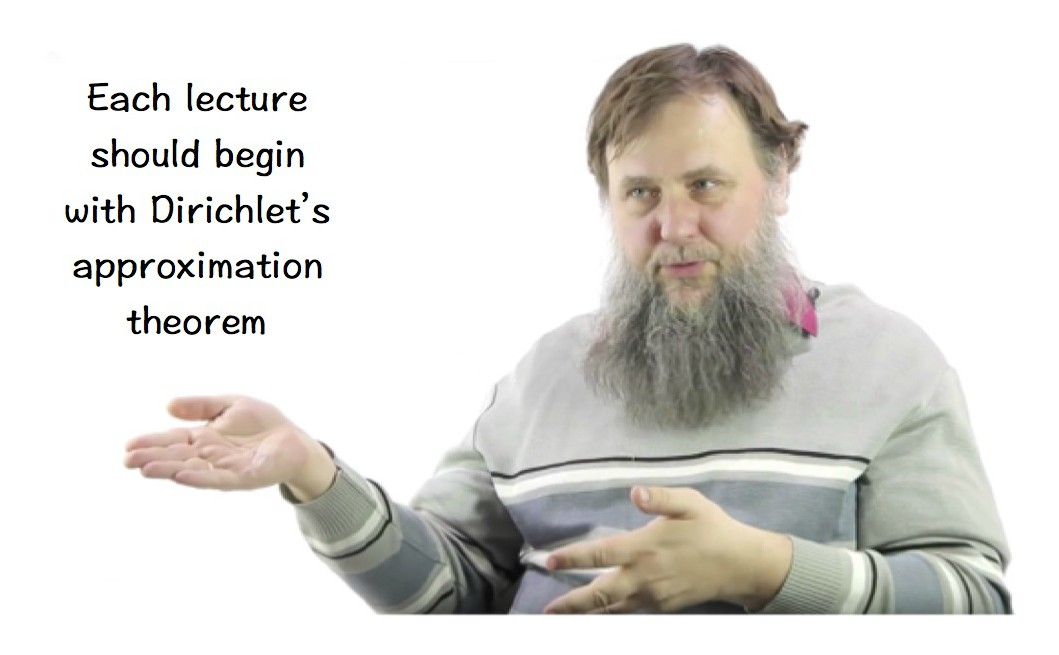
\includegraphics[width=\textwidth]{moschevitin}
    Действительно... Причём лекция может быть по любому предмету.
\end{figure}


\subsection{Предварительные сведения}
\label{subsec:III-1}

Пусть $\theta \in \RR$. Вопрос: насколько маленькой можно сделать разность $\abs{\theta - \frac{p}{q}}$ так, чтобы $\abs{\theta - \frac{p}{q}} < f(a)$ ($p$ и $q$ --- не простые).

\emph{Характеристикой} $\theta$ является то, насколько хорошо она приближается дробью $\frac{p}{q}$. Мы, конечно, знаем, что существуют нерациональные числа ($\sqrt{2}, \sqrt{3}, \dots$). Легко доказать, что корни многочленов с целыми коэффициентами (алгебраические числа, их множество обозначается как \AA) не будут рациональными.

Например, $\phi = \frac{1 + \sqrt{5}}{2}$ --- корень многочлена $x^2 - x - 1 = 0$, а его корни имею вид $\frac{\text{делитель} - 1}{\text{делитель} + 1} \in \{ \pm 1 \}$. Естественно, ни $1$, ни $-1$ корнями не являются.

А вдруг все числа алгебраические? Нет, алгебраических чисел счётное количество. Это доказал Лиувилль через теорию приближений: он показал, что алгебраические числа не могут приближаться ``слишком хорошо''.

То есть, для алгебраических чисел не найдётся такой функции $f$, для которой будет бесконечно много решений.

\begin{nstatement}
\label{stm:III-1}
    Если $\theta = \frac{a}{b} \in \RR$, то
    \[
        \forall \frac{p}{q} \in \QQ \setminus \{ 0 \}\colon \abs{\theta - \frac{p}{q}} > \frac{\sfrac{1}{b}}{q}.
    \]
\end{nstatement}
\begin{proof}
    \[
        \abs{\frac{a}{b} - \frac{p}{q}} = \frac{\abs{aq - bp}}{bq} \ge \frac{1}{bq},
    \] 
    так как $\abs{aq - bp} \in \ZZ\, \ne 0$.
\end{proof}

\begin{ntheorem}[Дирихле о приближении]
\label{thm:III-1}
    Пусть $\theta \in \RR$, $T \in \NN$. Тогда
    \[
        \exists \frac{p}{q} \in \QQ\colon \abs{\theta - \frac{p}{q}} < \frac{1}{qT},
        \quad
        1 \le q \le T.
    \]
\end{ntheorem}
\begin{proof}
    Хотим получить, что $\abs{q\theta - p} < \frac{1}{T}$. Можно считать, что $\theta \in [0, 1)$, и потом просто прибавить целую часть.~\newline
    Рассмотрим числа $\{ n\theta \}$, где $n = 0, 1, \dots, T$. Разобьём отрезок $[0, 1]$ на полуинтервалы $\left[ \frac{k}{T}, \frac{k+1}{T} \right)$, $k = 0, 1, \dots, T-1$ (то есть, на $T$ равных). По принципу Дирихле
    \[
        \exists n_1, n_2\colon 
        \left( n_1 - n_2 \right)\theta - \left( \left[ n_1\theta \right] - \left[ n_2\theta \right] \right) < 
        \frac{1}{T}.
    \]
    Остаётся положить $q = n_1 - n_2$, $p = \left[ n_1\theta \right] - \left[ n_2\theta \right]$. Тогда $q \ge 1$, $q \le T$ (то есть, $n_1, n_2 \le T$).
\end{proof}

\begin{ncorollary}
\label{crl:III-1}
    Если $\theta \in \RR \setminus \QQ$, то неравенство
    \[
        \abs{\theta - \frac{p}{q}} < \frac{1}{q^2}
    \]
    имеет бесконечно много решений в $\frac{p}{q} \in \QQ$.
\end{ncorollary}
\begin{proof}
    Докажем от противного: пусть $\frac{p_1}{q_1}, \frac{p_2}{q_2}, \dots, \frac{p_k}{q_k}$ --- все решения $\abs{\theta - \frac{p}{q}} < \frac{1}{q^2}$. 
    Положим $\delta = \min_i \abs{\theta - \frac{p_i}{q_i}} > 0$, $T = \left\lceil \frac{1}{\delta} \right\rceil$ (любое $T > \frac{1}{\delta}$). 
    По Теореме~\ref{thm:III-1} Дирихле 
    \[
        \exists \frac{p}{q},\, q \le T\colon \abs{\theta - \frac{p}{q}} < \frac{1}{qT} \le \frac{1}{q^2}.
    \]
    То есть $\frac{p}{q}$ должна быть среди дробей $\frac{p_i}{q_i}$. Но
    \[
        \abs{\theta - \frac{p}{q}} < \frac{1}{qT} < \frac{\delta}{q} \le \delta.
    \]
    Таким образом, $\frac{p}{q}$ ``ближе'', чем наименьшее $\delta$ --- пришли к противоречию.
\end{proof}

\begin{ndefinition}
\label{def:III_measure-of-irrationality}
    \emph{Мерой иррациональности} числа $\theta$ называют
    \[
        \mu(\theta) := \sup_s\colon \left\{ \abs{\theta - \frac{p}{q}} < \frac{1}{q^s} \text{ имеет бесконечно много решений } \frac{p}{q} \right\}.
    \]
\end{ndefinition}

\begin{remark}
    В качестве $\frac{p}{q}$ можно брать подходящие дроби в разложении $\theta$ в цепную дробь.
\end{remark}

    \end{lecture}

    \begin{lecture}{31 октября 2017 г.}
        \begin{ndefinition}
\label{def:III_badly-approximable}
    Иррациональное число $\theta$ называется \emph{плохо приближаемым}, если 
    \[
        \exists C = C(\theta) > 0\ \forall \frac{p}{q}\colon \ \abs{\theta - \frac{p}{q}} \ge \frac{C}{q^2}.
    \]
\end{ndefinition}

\begin{remark}
    Известно (существует такая теорема), что число плохо приближаемо тогда и только тогда, когда неполные частные при разложении в цепную дробь ограничены. Например, для квадратичной иррациональности неполные частные периодичны \footnote{По Теореме Лагранжа с первого курса}, а значит и ограничены, то есть квадратичные иррациональности плохо приближаемы.
\end{remark}

\begin{remark}
    Отныне и далее мы будем подразумевать, что $\theta \in \RR$, а $\alpha \in \CC$.
\end{remark}

\begin{ndefinition}
\label{def:III_algebraic-number}
    Число $\alpha \in \CC$ называется \emph{алгебраическим}, если существует ненулевой многочлен $f(x) \in \QQ[x] \setminus \{ 0\}$ такой, что
    \[
        f(\alpha) = 0.
    \]
    Такой многочлен $f(x)$ называется \emph{аннулирующим} для числа $\alpha$.
\end{ndefinition}

\begin{ndefinition}
\label{def:III_algebraic-number-degree}
    \emph{Степенью алгебраического числа} $\deg{\alpha}$ называется минимальная степень аннулирующего многочлена:
    \[
        \deg{\alpha} := \min\left\{ \deg{f} \mid f(x) \in \QQ[x] \setminus \{ 0 \},\, f(x) = 0 \right\}.
    \]
\end{ndefinition}

\begin{ntheorem}[Лиувилля]
\label{thm:III_Liouville}
    Пусть $\theta \in \RR$ --- алгебраическое число степени $d$. Тогда
    \[
        \exists C = C(\theta) > 0\ \forall \frac{p}{q} \in \QQ \setminus \{ 0 \}\colon \ \abs{\theta - \frac{p}{q}} \ge \frac{C}{q^d}.
    \]
    То есть $\mu(\theta) \le d$.
\end{ntheorem}
\begin{proof}
    \hfill
    \begin{casesp}
        \item
        $\theta \in \QQ$. 
            Случай $d = 1$ ($\theta \in \QQ$) уже был нами рассмотрен и доказан в Утверждении~\ref{stm:III-1}.
        \item
        $\theta \not\in \QQ$. 
            Рассмотрим многочлен $f(x) \in \ZZ[x] \setminus \{ 0 \}$, $\deg{f} = d \ge 2$, $f(\theta) = 0$. Заметим, что для любой $\frac{p}{q} \in \QQ$ справедливо $f\left(\frac{p}{q}\right) \ne 0$. Действительно, так как иначе многочлен $g(x) = \frac{f(x)}{x - \sfrac{p}{q}}$ был бы аннулирующим многочленом для $\theta$ степени $\deg{g} = \deg{f} - 1 = d - 1$. Пришли к противоречию.~\newline
            Поскольку многочлен $f(x)$ с целыми коэффициентами, то 
            \[
                q^d f\left(\frac{p}{q}\right) \in \ZZ \ \Rightarrow \ 
                \abs{q^d f\left(\frac{p}{q}\right)} \ge 1 \ \Rightarrow \ 
                \abs{f\left(\frac{p}{q}\right)} \ge \frac{1}{q^d}.
            \]
            \begin{casesp}
                \item
                $\abs{\theta - \frac{p}{q}} \ge 1$,
                    \[
                        \forall \frac{p}{q}\colon \ \abs{\theta - \frac{p}{q}} \ge \frac{1}{q^d}.
                    \]
                \item
                $\abs{\theta - \frac{p}{q}} < 1$, то есть $\frac{p}{q} \in [\theta - 1, \theta + 1]$. 
                    \begin{align*}
                        \frac{1}{q^d} &\le \abs{f\left(\frac{p}{q}\right)} = \abs{f\left(\frac{p}{q}\right) - f\left(\theta\right)} \\
                        &= \abs{\left(\frac{p}{q} - \theta\right)f'(\xi)} \le M \cdot \abs{\theta - \frac{p}{q}},
                    \end{align*}
                    где $M = \max_{[\theta-1, \theta+1]} \abs{f'(x)}$. Таким образом, $\abs{\theta - \frac{p}{q}} \ge \frac{1}{Mq^d}$.~\newline
                    Следовательно, 
                    \[
                        C = \min\left( 1, \frac{1}{M} \right).
                    \]
            \end{casesp}
    \end{casesp}
\end{proof}    

\begin{ndefinition}
\label{def:III_Liouville-number}
    Если $\theta \in \RR$ таково, что $\forall n \in \NN$ неравенство $\abs{\theta - \frac{p}{q}} < \frac{1}{q^n}$ имеет бесконечное количество решений в $\frac{p}{q} \in \QQ$, то число $\theta$  называется \emph{луивиллевым} (или \emph{числом Луивилля}.
\end{ndefinition}

\begin{ndefinition}
\label{def:III_Diophantine-number}
     Числа, не являющиеся луивиллевыми, называются \emph{диофантовыми}.
\end{ndefinition}

\begin{proposition}
\label{pr:III-1}
    Луивиллевы числа трансцендентны.
\end{proposition}
\begin{proof}
    Предположим противное --- пусть $\theta$ алгебраическое. Тогда для него верна Теорема~\ref{thm:III_Liouville} Луивилля:
    \[
        \exists C > 0\ \forall \frac{p}{q} \in \QQ \setminus \{ 0 \}\colon \ \abs{\theta - \frac{p}{q}} \ge \frac{C}{q^d}.
    \] 
    Тогда при $n \ge d$ из неравенства 
    \[
        \abs{\theta - \frac{p}{q}} < \frac{1}{q^{n + 1}}
    \]
    следует, что $q \le \frac{1}{C}$. Кроме того, 
    \[
        \abs{q\theta - p} \le 1 \ \Rightarrow \ 
        \abs{p} \le 1 + q\abs{\theta} < 1 + \frac{\abs{\theta}}{C}.
    \]
    То есть числа $q$ и $p$ ограничены, значит и количество решений тоже --- получили противоречие.
\end{proof}

\begin{example}
    Число $\theta = \sum_{n=0}^{\infty} \frac{1}{2^{n!}}$ --- луивиллево.
\end{example}
\begin{proof}
    Пусть $m \in \NN$, $N \ge m$. Положим 
    \[
        p = 2^{N!} \sum_{n=0}^{N} \frac{1}{2^{n!}}, 
        \quad 
        q = 2^{N!}.
    \]
    Тогда
    \[
        \frac{p}{q} = \sum_{n=0}^{N} \frac{1}{2^{n!}},
    \]
    а следовательно,
    \begin{align*}
        \abs{\theta - \frac{p}{q}} &= \sum_{n=N+1}^{\infty} \frac{1}{2^{n!}} 
          \le \frac{1}{2^{(N+1)!}}\left( 1 + \frac{1}{2^{(N+2)! - (N+1)!}} + \frac{1}{2^{(N+3)! - (N+1)!}} + \dots \right) \\
          &< \frac{1}{2^{(N+1)!}}\left( 1 + \frac{1}{2} + \frac{1}{4} + \dots \right) = \frac{2}{2^{(N+1)!}} \\
          &= \frac{2}{q^{N+1}} \le \frac{1}{q^N} \le \frac{1}{q^m}.
    \end{align*}
    Таким образом, неравенство 
    \[
        \abs{\theta - \frac{p}{q}} 
        = \abs{\theta - \frac{2^{N!} \sum_{n=0}^{N} \frac{1}{2^{n!}}}{2^{N!}}} 
        < \frac{1}{q^m}
    \]
    имеет бесконечное число решений.
\end{proof}

Кругозора ради добавим, что существует следующая очень сложная Теорема:

\begin{ntheorem}[Туэ--Зигеля--Рота]
\label{thm:III_Thue-Siegel-Roth}
    Пусть $\theta$ --- иррациональное алгебраическое число. Тогда 
    \[
        \forall \epsilon > 0 \ \exists C = C(\theta, \epsilon)\colon \forall \frac{p}{q} \in \QQ\ \abs{\theta - \frac{p}{q}} \ge \frac{C}{q^{2 + \epsilon}} = \frac{2}{q^{N+1}} \le \frac{1}{q^N} \le \frac{1}{q^m}.
    \]
    Таким образом, неравенство $\abs{\theta - \frac{p}{q}} \le \frac{1}{q^m}$ имеет бесконечное количество решений.
\end{ntheorem}


\subsection{\texorpdfstring{Иррациональность $e$ и $\pi$}{Иррациональность e и π}}
\label{subsec:III-2}

\begin{ntheorem}
\label{thm:III_E-irrationality}
    $e \not\in \QQ$.
\end{ntheorem}
\begin{proof}
    Вспомним первый семестр курса математического анализа:
    \[
        e = \sum_{n=0}^{\infty} \frac{1}{n!}.
    \]
    Допустим противное: пусть $e = \frac{p}{q} \in \QQ$. Тогда 
    \[
        q!e \in \NN.
    \]
    Несложно тогда заметить, что 
    \begin{align*}
        \NN \ni \sum_{n=q+1}^{\infty} \frac{q!}{n!} &= \frac{1}{q+1} + \frac{1}{(q+1)(q+2)} + \frac{1}{(q+1)(q+2)(q+3)} + \dots \\
        &< \sum_{k=1}^{\infty} \frac{1}{(q+1)^k} = \frac{1}{q} \\
        &\le 1.
    \end{align*}
    Получили противоречие.
\end{proof}

\begin{ntheorem}
\label{thm:III_PI-irrationality}
    $\pi \not \in \QQ$.
\end{ntheorem}
\begin{proof}
    Снова допустим противное: пусть $\pi = \frac{p}{q} \in \QQ$. Тогда положим 
    \begin{align*}
        f_n(x) &= q^n\frac{x^n (\pi - x)^n}{n!} = \frac{x^n(q - px)^n}{n!} \\
        &= \frac{q(x)}{n!}, \quad g(x) \in \ZZ[x].
    \end{align*}
    Далее рассмотрим
    \[
        I_n = \int_{0}^{\pi} f_n(x)\sin(x)dx, \quad I_n \ge 0
    \]
    и
    \[
        F_n(x) = f_n(x) - f_n''(x) + f_n^{(4)}(x) + \dots = \sum_{k = 0}^{\infty} (-1)^k f_n^{(2k)}(x).
    \]
    Поскольку $f_n(x) = f_n(\pi-x)$, то при чётных $k$ справедливо
    \[
        f_n^{(k)}(x) = f_n^{(k)}(\pi - x).
    \]
    Из этого мы видим, что $F_n(x) = F_n(\pi - x)$. Тогда
    \[
        \left( F_n'(x)\sin{x} - F_n(x)\cos{x} \right)' = f_n(x)\sin x.
    \]
    А следовательно,
    \[
        I_n = \left( F_n'(x)\sin{x} - F_n(x)\cos{x} \right)\Bigr|_0^\pi = F_n(0) + F_n(\pi) = 2F_n(0).
    \]
    Докажем теперь следующие (взаимоисключающие) утверждения про такой интеграл:
    \begin{enumerate}
        \item $I_n > 0$.
        \item $I_n \to 0$ при $n \to \infty$.
        \item $I_n \in \ZZ$ при $n \in \NN$.
    \end{enumerate}
    \begin{statesp}
        \item
            Очевидно.
        \item
            \[
                \abs{f_n(x)\sin{x}} \le \frac{b^n\left( \sfrac{\pi}{2} \right)^{2n}}{n!} \xrightarrow{n \to \infty} 0.
            \]
        \item
            \[
                I_n = 2F_n(0) = 2 \sum_{k=0}^{\infty} (-1)^k, \quad f^{(2k)}(0) \in \ZZ.
            \]
            Поясним, что $f^{(2k)}(0) \in \ZZ$, так как при $g(x) \in \ZZ[x]$ и $l \ge n$ выполняется $\frac{g^{(l)}(x)}{n!} \in \ZZ[x]$.
    \end{statesp}
    Таким образом, пришли к тому, что последовательность $\left\{ I_n \right\}$ положительна, целочисленна, и стремится к нулю одновременно. То есть к противоречию.
\end{proof}

    \end{lecture}

    \begin{lecture}{7 ноября 2017 г.}
        \subsection{\texorpdfstring{Трансцендентность числа $e$}{Трансцендентность числа e}}
\label{III_E-transcendental}

\begin{ntheorem}
    Число $e$ трансцендентно.
\end{ntheorem}
\begin{proof}
    Предположим противное: пусть $e$ --- алгебраическое число степени $m$. В таком случае
    \[
        \exists a_0, a_1, \dots, a_m \in \ZZ\colon \sum_{k=0}^m a_ke^k = 0,\, \exists k\colon a_k \ne 0.
    \]
    Можно считать, что $\left( a_0, a_1, \dots, a_m \right) = 1$. Ортогональным дополнением к вектору ${\left( a_0, a_1 \dots, a_m \right)}$ является гиперплоскость $\Pi$, проходящая через $\left( 1, e, e^2, \dots, e^m \right)$ (Рис.~\ref{fg:IV-1}). При этом в гиперплоскости можно выбрать базис из целочисленных векторов.
    \begin{figure}[h]
        \centering
        % First illustration of the orthogonal complement used in the proof of Theorem III.6 (the transcendentality of E)
% See Lecture 10
\tikz[cm={cos(-18),-sin(-18),sin(-18),cos(-18),(0,0)}]{
    % Sets the axes
    \draw[thick,->]
        (0, 0) -- (0, 1.5) 
        node[anchor=south east]{$\left( a_0, a_1, \dots, a_m \right)$};
    \draw[thick,->] 
        (0, 0) -- (1.5, 0) 
        node[anchor=south west]{$\left( 1, e, e^2, \dots, e^m \right)$};
    % Draws the origin point
    \filldraw 
        (0, 0) circle (1.8pt) 
        node[anchor=north east]{$O$};
    % Draws the right angle
    \draw
        (0, 0.32) -- (0.32, 0.32) -- (0.32, 0);
}

        \caption{Ортогональное дополнение к $\left( a_0, a_1 \dots, a_m \right)$}
        \label{fg:IV-1}
    \end{figure}

    Разбиваем все точки $\ZZ^{m+1}$ на параллельные слои $\ZZ^m$ (любое $b \in \ZZ^{m+1}$ лежит в соответствующем слое с номером $\langle a, b \rangle$) (Рис.~\ref{fg:IV-2}).
    
    \begin{figure}[!ht]
        \centering
        % Second illustration of the orthogonal complement used in the proof of Theorem III.6 (the transcendentality of E)
% See Lecture 10
\tikz[ultra thin,cm={cos(90),-sin(90),sin(90),cos(90),(0,0)}]{
    % Sets the bottom hyperplane
    \node[trapezium,trapezium left angle=100,trapezium right angle=80,minimum width=3.2cm,minimum height=2cm,fill=blue!45,opacity=0.48] at (1, 1){};
    % Sets the middle hyperplane (the orthogonal complement itself)
    \node[trapezium,trapezium left angle=100,trapezium right angle=80,minimum width=3.2cm, minimum height=2cm,fill=blue!45,opacity=0.48] at (0.5, 0.5){};
    \draw[thick,->]
        (1.37, -0.5) -- (1.37, 1.8)
        node[anchor=north west]{$\left( 1, e, e^2, \dots, e^m \right)$};
    % Sets the top hyperplane
    \node[trapezium,trapezium left angle=100,trapezium right angle=80,minimum width=3.2cm,minimum height=2cm,fill=blue!45,opacity=0.48] at (0, 0){};
    % Sets the hyperplane's label
    \draw
        (0.3, 1.7)
        node[anchor=north west]{$\Pi$}
}

        \caption{Расслоение $\ZZ^{m+1}$}
        \label{fg:IV-2}
    \end{figure}
    
    Расстояние между слоями одинаковое и (при условии, что $(a_0, a_1, \dots, a_m) = 1$) оно равно $\Delta := \frac{1}{\sqrt{a_0^2 + a_1^2 + \dots + a_m^2}}$. Построим последовательность $\mathcal{B}^{(n)} \in \ZZ^{m+1}$ такую, что
    \begin{enumerate}
        \item
            расстояние от $\mathcal{B}^{(n)}$ до $\left< \left(1, e, e^2, \dots, e^m \right) \right>$ меньше $\Delta$,
        \item
            точка $\mathcal{B}^{(n)}$ не лежит в гиперплоскости $\Pi$.
    \end{enumerate}
    Напомним четвёртый семестр курса математического анализа:
    \[
        \int_{0}^{\infty} x^ke^{-x}dx = \Gamma(k+1) = k!
    \]
    Тогда можно брать $\int_{0}^{\infty} f(x)e^{-x}dx$ для многочленов $f$. Положим 
    \[
        f_n(x) = \frac{x^{n-1}(x-1)^n(x-2)^n \dots (x-m)^n}{(n-1)!}.
    \]
    Возьмём
    \[
        \mathcal{B}_k^{(n)} = \int_{0}^{+\infty} f_n(x+k)e^{-x}dx,
        \quad 
        k = 0, 1, \dots, m.
    \]
    Покажем справедливость следующего Утверждения:
    \begin{statement}
        \[
            \mathcal{B}_0^{(n)}e^k - \mathcal{B}_k^{(n)} \to 0,\ n \to \infty.
        \]
    \end{statement}
    \begin{proof}
    \hfill
        \begin{casesp}
            \item
            $k = 0$.
                В этом случае разность будет равна нулю.
            \item
            $k \ne 0$. Обозначим $y = x + k$.
                \begin{align*} 
                    \abs{\mathcal{B}_0^{(n)}e^k - \mathcal{B}_k^{(n)}} 
                    &= \abs{e^k \int_{0}^{\infty} f_n(x)e^{-x}dx - \int_{0}^{\infty} f_n(x + k)e^{-x}dx} \\
                    &= e^k \abs{\int_{0}^{\infty} f_n(x)e^{-x}dx - \int_{k}^{\infty} f_n(y)e^{-y}dy} \\
                    &= e^k \abs{\int_{0}^{k} f_n(x)e^{-x}dx} \\
                    &\le e^m m \frac{m^{n+nm-1}}{(n-1)!} = \frac{e^m m^{n(1+m)}}{(n-1)!} \xrightarrow{n \to \infty} 0.
                \end{align*}
        \end{casesp}
    \end{proof}
    \noindent
    Таким образом, мы показали справедливость нашего Утверждения. А это означает, что последовательность точек $\mathcal{B}^{(n)}$ стремится к прямой $\left< \left( 1, e, e^2, \dots, e^m \right) \right>$ и, начиная с некоторого $n$, расстояние между ними станет меньше $\Delta$.~\newline
    Покажем теперь, что $\mathcal{B}_k^{(n)} \in \ZZ$, где $k = 0, \dots, m$:
    \begin{casesp}
        \item
        $k = 0$.
            \begin{align*}
                \mathcal{B}_0^{(n)} 
                 &= \frac{1}{(n-1)!} \sum_k \left( \left[\text{коэффициент в } x^{n-1}(x-1)^n \dots (x-m)^n \text{ при } x^k \right] \cdot \right. \\
                 &\phantom{= \frac{1}{(n-1)!} \sum_k} \left. \cdot \int_{0}^{\infty} x^ke^{-x}dx \right) \\
                &= \frac{1}{(n-1)!}\left( (-1)^{mn} m!^n (n-1)! + A_n n! + \dots + A_N N! \right) \\
                &= (-1)^{mn}m!^n + nA,\, A \in \ZZ.
            \end{align*}
        \item
        $k \ge 1$:
            \begin{align*}
                \mathcal{B}_k^{(n)}
                 &= \int_{0}^{+\infty}f_n(x+k)e^{-x}dx \\
                 &= \sum_j \left( \left[\text{коэффициент в } \frac{(x+k)^{n-1}(x+k-1)^n \dots x^n \dots}{(n-1)!} \text{ при } x^j \right] \cdot j! \right) \\
                 &= \frac{1}{(n-1)!}\left( C_nn! + C_{n+1}(n+1)! + \dots + C_NN! \right) = nC,\, C \in \ZZ.
            \end{align*}
    \end{casesp}
    Осталось показать, что для бесконечно многих $n$ справедливо, что $\mathcal{B}^{(n)} \not\in \Pi$. То есть что
    \[
        \sum_{k=0}^{m} a_k \mathcal{B}_k^{(n)} \ne 0.
    \]
    Для этого обратим внимание на следующее сравнение:
    \[
        \congr{\sum_{k=0}^m a_k \mathcal{B}_k^{(n)}}
          {a_0(-1)^{mn} {m!}^n}
          {n}.
    \]
    Тогда при $\gcd{n, a_0m!} = 1$, где $a_0m!$ --- некоторое фиксированное число, ряд как раз и станет отличным от нуля.
\end{proof}



\section{Алгебраические и трансцендентные числа}
\label{sec:IV_algebraic-transcendental-numbers}


\subsection{Основные сведения}
\label{subsec:1_summary}

\begin{remark}
    Как уже упоминалось ранее, множество алгебраических чисел обозначается через \AA.
\end{remark}

Пусть заданы некоторый многочлен $f(x) \in \QQ[x]$ и $\alpha \in \AA$. Далее, пусть $f(\alpha) = 0$, $\deg{f} = \deg{\alpha}$. Тогда $f(x)$ неприводим над $\QQ$. Следовательно, если 
\[
    g(x) \in \QQ[x],\, g(\alpha) = 0,\, \deg{g} = \deg{\alpha} = \deg{f},
\]
то $\gcd{f(x), g(x)} = h(x) \in \QQ[x]$, при этом $h(\alpha) = 0 = \deg{h} = \deg{f}$. То есть, если $h$ делит $f$ и $g$, а $\deg{h} = \deg{f} = \deg{g}$, то все три являются пропорциональными:
\[
    f \sim g \sim h.
\]

\begin{ndefinition}
\label{def:IV_minimal-polynomial}
    Унитарный многочлен\footnote{То есть многочлен, старший член которого равен единице.} $p_\alpha(x) \in \QQ[x]$ называется \emph{минимальным многочленом $\alpha$}, если
    \[
        p_\alpha(\alpha) = 0, \quad \deg{p_\alpha} = \deg{\alpha}.
    \]
\end{ndefinition}

\begin{theorem}[Алгебраическая замкнутость поля \AA]
    Поле \AA~--- алгебраически замкнутое поле. Иными словами, корень многочлена с алгебраическими коэффициентами также алгебраическое число.
\end{theorem}

Для доказательства этой Теоремы нам сперва понадобится установить несколько дополнительных фактов и лемм.

\begin{ntheorem}[О симметрических многочленах]
\label{thm:IV-1}
    Пусть \rr~--- ассоциативное коммутативное кольцо с единицей и без делителей нуля. Далее, пусть многочлен $f \left( x_1, x_2, \dots, x_m \right) \in \rr\left[ x_1, x_2, \dots, x_m \right]$ является симметрическим. Тогда 
    \begin{align*}
        \exists g\left( x_1, x_2, \dots x_m \right) &\in \rr\left[ x_1, x_2, \dots, x_m \right]\colon \\
        f\left( x_1, x_2, \dots, x_m \right) &= g\left( s_1\left( x_1, x_2, \dots, x_m \right), \dots, s_m\left( x_1, x_2, \dots, x_m \right) \right),
    \end{align*}
    где $s_k\left( x_1, x_2, \dots, x_m \right)$ --- $k$-ый симметрический многочлен.
\end{ntheorem}

\begin{nlemma}
\label{lm:IV-1}
    Пусть $f(x,y) \in \rr[x, y]$, тогда
    \begin{align*}
        \exists g(x, y_1, \dots, y_m) &\in \rr[x, y_1, \dots, y_m]\colon \\
        \prod_{i=1}^{m} f(x, y_i) &= g(x, s_1(y_1, \dots, y_m), \dots, s_m(y_1, \dots, y_m)).
    \end{align*}
\end{nlemma}
\begin{proof}
    Заметим, что
    \[
        \prod_{i=1}^{m} f(x, y_i) \in \rr[x][y_1, y_2, \dots, y_m].
    \]
    Таким образом, он является симметрическим по $y_1, y_2, \dots, y_m$ над кольцом $\rr[x]$. По Теореме~\ref{thm:IV-1} существует искомый многочлен $g$, причём $g$ --- многочлен от $(x, y_1, \dots, y_m)$ над $\rr$:
    \[
        \exists g \in \rr[x][y_1, y_2, \dots, y_m]\colon g\left( s_1\left( y_1, \dots, y_m \right), \dots, s_m\left( y_1, \dots, y_m \right) \right) = 0.
    \]
\end{proof}

\begin{nlemma}
\label{lm:IV-2}
    Пусть многочлен $f(x,y) \in \QQ[x, y]$, элемент $\alpha \in \AA$, $\deg{\alpha} = n$, $\alpha_1 = \alpha$, $\alpha_2, \alpha_3, \dots, \alpha_n$ --- корни многочлена $p_\alpha(x)$\footnote{Они попарно различны как корни любого неприводимого многочлена $f(x)$. Иначе бы у $f'(x)$ и $f(x)$ был общий корень, но $\deg{f'} < \deg{f}$ --- противоречие с неприводимостью.}. Тогда 
    \[
        F(x) = \prod_{k=1}^n f(x, \alpha_k) \in \QQ[x].
    \]
\end{nlemma}
\begin{proof}
    Применим Лемму~\ref{lm:IV-1}:
    \[
        \prod_{k=1}^n f(x, \alpha_k) = g\left( s_1\left( \alpha_1, \dots, \alpha_n \right), \dots, s_n\left( \alpha_1, \dots, \alpha_n \right) \right).
    \]
    По Теореме Виета все $s_i(\alpha_1,\dots,\alpha_n)$ выражаются через коэффициенты многочлена $p_\alpha$. А следовательно, для каждого индекса $i$ справедливо $s_i(\alpha_1, \dots, \alpha_n) \in \QQ$.
\end{proof}

\begin{ntheorem}
\label{thm:IV-2}
    \AA --- поле.
\end{ntheorem}
\begin{proof}
    Пусть $\alpha, \beta \in \AA$. Проверяем, что $\left\{ \alpha @ \beta \in \AA \mid @ \in \{+, -, /, \cdot \} \right\}$.
    \begin{statesp}
        \item[($+$):]
            Рассмотрим $F_1(x) = \prod_{k=1}^m p_\alpha\left( x-\beta_k \right)$, где $\beta_1 = \beta, \beta_2, \dots, \beta_m$ --- корни $p_\beta(x)$. Тогда по Лемме~\ref{lm:IV-2}:
            \[
                F_1(x) \in \QQ[x].
            \]
            При этом 
            \[
                F_1(\alpha + \beta) = \ldots \cdot p_\alpha(\alpha + \beta - \beta) \cdot \ldots = 0.
            \]
        \item[($-$):]
            Если $\beta$ --- алгебраическое число, то алгебраическим будет и $-\beta$. Тогда $\alpha - \beta$ -- тоже алгебраическое. Ну или так:
            \[
                F_2(x) = \prod_{k=1}^m p_\alpha \left( x + \beta \right) \in \QQ[x], \quad F_2(\alpha - \beta) = 0.
            \]
        \item[($/$):]
            \[
                F_3(x) = \prod_{k=1}^m p_\alpha\left( x\beta_k \right) \in \QQ[x], \quad F_3\left( \frac{\alpha}{\beta} \right) = 0.
            \]
        \item[($\cdot$):]
            \[
                F_4(x) = \prod_{k=1}^m \beta_k^m p_\alpha\left( \frac{x}{\beta_k} \right) \in \QQ[x], \quad F_4\left( \alpha\beta \right) = 0.
            \]
    \end{statesp}
\end{proof}

    \end{lecture}

    \begin{lecture}{14 ноября 2017 г.}
        \subsection{Целые алгебраические числа}
\label{subsec:IV-2}

\begin{ndefinition}
\label{def:IV_algebraic-integer}
    Алгебраическое число $\alpha$ называется \emph{целым алгебраическим}, если $p_{\alpha}(x) \in \ZZ[x]$, т.е. если $p_{\alpha}(x)$ имеет целые коэффициенты. Множество всех целых алгебраических чисел обозначим через $\ZZ_\AA$.
\end{ndefinition}

\begin{example}
\hfill
    \begin{enumerate}
        \item
            Пусть $\alpha \in \QQ$. Тогда $\alpha \in \ZZ_\AA \Leftrightarrow \alpha \in \ZZ$;
        \item
            $\sqrt{2} \in \ZZ_\AA$;
        \item
            $a, b, d \in \ZZ \ \Rightarrow \ a + b\sqrt{d} \ZZ_\AA$;
        \item
            $\frac{1 + \sqrt{5}}{2} \in \ZZ_\AA$.
    \end{enumerate}
\end{example}

\begin{remark}[Анонс!]
    Почему $\ZZ_\AA$ --- кольцо? Нужно смотреть в сторону доказательства Теоремы~\ref{thm:IV-2}. Для $\alpha \pm \beta$ и $\alpha\beta$ мы построили какие-то многочлены из $\ZZ[x]$ со старшим членом равным единице, которые обнуляют $\alpha \pm \beta$ и $\alpha\beta$ соответственно. А в Определении~\ref{def:IV_algebraic-integer} --- минимальный многочлен (а не какой-то там). Вопрос: можно ли выкинуть из Определения слово ``минимальный''? Оказывается, что можно, и это будет следовать из Леммы~\ref{lm:IV-3} Гаусса.
\end{remark}

\begin{ndefinition}
\label{def:IV_primitive-polynomial}
    Многочлен 
    \[
        f(x) = a_nx^n + a_{n-1}x^{n-1} + \dots + a_1x + a_0 \in \ZZ[x]
    \]
    называется \emph{примитивным}, если $\gcd{a_n, a_{n-1}, \dots, a_1, a_0} = 1$.
\end{ndefinition}

\begin{nlemma}[Гаусса]
\label{lm:IV-3}
    Произведение примитивных многочленов примитивно.
\end{nlemma}
\begin{proof}
    Рассмотрим следующие примитивные многочлены:
    \begin{align*}
        f(x) &= a_nx^n + a_{n-1}x^{n-1} + \dots + a_1x + a_0, \\
        g(x) &= b_mx^m + b_{m-1}x^{m-1} + \dots + b_1x + b_0.
    \end{align*}
    А также введём многочлен
    \[
        h(x) := f(x)g(x) = c_{m+n}x^{m+n} + c_{m+n-1}x^{m+n-1} + \dots + c_1x + c_0.
    \]
    Допустим противное: пусть существует такое простое $p$, что $\forall 0 \le k \le m + n\colon p \divides c_k$. Пусть 
    \[
        r = \min\left\{k \mid p \notdivides a_k\right\},
        \quad
        s = \min\left\{k \mid p \notdivides b_k\right\}.
    \]
    Но тогда 
    \[
        c_{r+s} = \sum_{i+j=r+s} a_ib_j = \notcongr{a_rb_s}{0}{p}.
    \]
    То есть получается, что $p \notdivides c_{r+s}$. Противоречие.
\end{proof}

\begin{ntheorem}
\label{thm:IV-3}
    Если существует унитарный многочлен
    \[
        f(x) \ne 0 \in \ZZ[x]\colon f(\alpha) = 0,
    \]
    то $\alpha \in \ZZ_\AA$.
\end{ntheorem}
\begin{proof}
    Заметим, что $p_{\alpha}(x) \divides f(x)$ в $\QQ[x]$, иными словами
    \[
        \exists g(x) \in \QQ[x]\colon f(x) = g(x)p_{\alpha}(x).
    \]
    Так как многочлены $f(x)$ и $p_{\alpha}(x)$ оба унитарные, то старший коэффициент $g(x)$ равен единице.~\newline
    Покажем, что  $g(x), p_{\alpha}(x) \in \ZZ[x]$. Пусть $A, B$ --- НОК знаменателей коэффициентов $g(x)$ и $p_{\alpha}(x)$ соответственно. Тогда $Ag(x)$ и $Bp_{\alpha}(x)$ --- примитивные многочлены. Далее, многочлен
    \[
        ABf(x) = Ag(x)Bp_{\alpha}(x)
    \]
    является примитивным по Лемме~\ref{lm:IV-3} Гаусса. Тогда все коэффициенты $ABf(x)$ делятся на $AB$, а следовательно, $AB = 1$ и $A = B = 1$.~\newline
    Таким образом, мы доказали, что $p_{\alpha}(x) \in \ZZ[x]$, а значит, что $\alpha \in \ZZ_\AA$.
\end{proof}

\begin{nlemma}
\label{lm:IV-4}
    Пусть $f(x, y) \in \ZZ[x, y]$, $\alpha_1, \alpha_2 \dots, \alpha_n$ -- сопряжённые к $\alpha \in \ZZ_\AA$. Тогда
    \[
        F(x) = \prod_{i=1}^{n} f\left(x, \alpha_i\right) \in \ZZ[x].
    \]
\end{nlemma}
\begin{proof}
    Аналогично доказательству Леммы~\ref{lm:IV-2}.
\end{proof}

\begin{ntheorem}
\label{thm:IV-4}
    $\ZZ_\AA$ --- кольцо.
\end{ntheorem}
\begin{proof}
    Пусть $\alpha, \beta \in \ZZ_\AA$ и 
    \begin{align*}
        \alpha_1, \alpha_2, \dots, \alpha_n \\
        \beta_1, \beta_2, \dots, \beta_m
    \end{align*}
    сопряженные к $\alpha$ и $\beta$ соответственно.
    Тогда, по Лемме~\ref{lm:IV-4}
    \begin{align*}
        F_1(x) &= \prod_{i=1}^{m} p_{\alpha}(x - \beta_i) \in \ZZ[x], \\
        F_2(x) &= \prod_{i=1}^{m} p_{\alpha}(x + \beta_i) \in \ZZ[x], \\
        F_3(x) &= \prod_{i=1}^{m} \beta_i^{\deg{p_{\alpha}}} p_{\alpha}\left( \frac{x}{\beta_i} \right) \in \ZZ[x],
    \end{align*}
    причём все три многочлена являются унитарными и
    \[
        F_1(\alpha + \beta) = F_2(\alpha - \beta) = F_3(\alpha\beta) = 0.
    \]
    Для завершения доказательства остаётся применить Теорему~\ref{thm:IV-3}.
\end{proof}

\begin{nproblem}
\label{prb:IV-1}
    Доказать, что для каждого $\alpha \in \AA$ существует такое $d \in \ZZ$, что $d\alpha \in \ZZ_\AA$.
\end{nproblem}


\subsection{\texorpdfstring{Конечные расширения поля \QQ}{Конечные расширения поля Q}}
\label{subsec:IV-3}

\begin{remark}
    В этом параграфе подразумевается, что $\alpha_1, \alpha_2, \dots, \alpha_n$ --- произвольные алгебраические числа.
\end{remark}

\begin{ndefinition}
\label{def:IV-extension}
    \emph{Расширением} \QQ, порождённым числами $\alpha_1, \alpha_2, \dots, \alpha_n$ называется
    \[
        \QQ(\alpha_1, \alpha_2, \dots, \alpha_n) := 
        \left\{ 
          \frac{f(\alpha_1, \alpha_2, \dots, \alpha_n)}{g(\alpha_1, \alpha_2, \dots, \alpha_n)} 
        \bigg| 
          f, g \in \QQ\left[ x_1, \dots, x_n \right],\, 
          g(\alpha_1, \dots, \alpha_n) \ne 0 
        \right\}.
    \]
\end{ndefinition}

\begin{nproblem}
\label{prb:IV-2}
    Доказать, что $\QQ\left(\alpha_1, \alpha_2, \dots, \alpha_n\right)$ --- минимальное по включению поле, содержащее и $\QQ$, и $\alpha_1, \alpha_2, \dots, \alpha_n$.
\end{nproblem}

\begin{nlemma}
\label{lm:IV-5}
    Пусть $\EE = \QQ(\theta)$, где $\deg{\theta} = n$. Тогда любой элемент $\alpha \in \EE$ однозначно представим в виде
    \[
        \alpha = c_0 + c_1\theta + \dots + c_{n-1} \theta^{n-1},\ c_i \in \QQ.
    \]
\end{nlemma}
\begin{proof}
\hfill
    \begin{statesp}
        \item[($\exists$):]
            Рассмотрим $\alpha = \frac{f(\theta)}{g(\theta)} \in \EE$. Так как $g(\theta) \ne 0$, то ${\gcd{p_{\theta}(x), g(x)} = 1}$. Если записать формально, то
            \[
                \exists u(x), v(x) \in \QQ[x]\colon u(x) p_{\theta}(x) + v(x)g(x) = 1.
            \]
            Тогда $u(\theta) p_{\theta}(\theta) + v(\theta) g(\theta) = 1$. Поскольку первое слагаемое обращается в ноль из-за $p_{\theta}(\theta)$, то $\frac{1}{g(\theta)} = v(\theta)$ и, стало быть, $\alpha = f(\theta) g(\theta)$. Положим теперь ${h(x) = f(x)g(x)}$ и поделим $h(x)$ с остатком на $p_{\theta}(x)$:
            \[
                h(x) = q(x)p_{\theta}(x) + r(x),\ \deg{r(x)} < \deg{\theta},\, q(x), r(x) \in \QQ[x].
            \]
            Тогда подтверждаем представимость элемента $\alpha$ в искомом виде:
            \[
                \alpha = h(\theta) = r(\theta),\ \deg{r(x)} < n,\, r(x) \in \QQ[x].
            \]
        \item[($!$):]
            Пусть 
            \[
                \alpha = c_0 + c_1\theta + \dots + c_{n-1}\theta^{n-1} = d_0 + d_1\theta + \dots + d_{n-1}\theta^{n-1}.
            \]
            Тогда легко вывести обнуляющий многочлен $\theta$ степени не больше $\deg{\theta-1}$:
            \[
                (c_0-d_0) + (c_1-d_1)\theta + \dots + (c_{n-1}-d_{n-1})\theta^{n-1} = 0.
            \]
            Следовательно, по определению $\deg{\theta}$ получаем, что $\forall i\colon c_i = d_i$, а следовательно, представление единственно.
    \end{statesp}
\end{proof}

\begin{remark}
    Таким образом, $\QQ(\theta)$ --- линейное пространство над $\QQ$ размерности $n$ с базисом $1, \theta, \dots, \theta^{n-1}$.
\end{remark}

\begin{ntheorem}[О примитивном элементе]
\label{thm:IV-5}
    Пусть $\EE = \QQ(\alpha_1, \alpha_2, \dots, \alpha_n)$. Тогда
    \[
        \exists \theta \in \EE\colon \EE = \QQ(\theta).
    \]
\end{ntheorem}

\begin{ndefinition}
\label{def:IV_primitive-element}
    Число $\theta$ из Теоремы~\ref{thm:IV-5} называется \emph{примитивным элементом} \EE~над полем \QQ.
\end{ndefinition}

\begin{corollary}
    Любое конечное расширение \QQ~является конечномерным пространством над \QQ.
\end{corollary}
\begin{proof}
    Действительно, возьмём примитивный элемент --- по Лемме~\ref{lm:IV-4} его степень будь равна размерности.
\end{proof}

\begin{ndefinition}
\label{def:IV_extension-degree}
    Размерность \EE~как линейного пространства над \QQ~называется \emph{степенью расширения}. Обозначается как $\left[\EE : \QQ\right]$.
\end{ndefinition}

Обозначим $\ZZ_\EE := \EE \cap \ZZ_\AA$. В частности, $\ZZ_\QQ = \ZZ$.

    \end{lecture}

    \begin{lecture}{21 ноября 2017 г.}
        \begin{proof}[Доказательство Теоремы~\ref{thm:IV-5}]
    Нам достаточно доказать утверждение Теоремы лишь для двух алгебраических чисел. То есть мы рассматриваем случай, когда $\EE = \QQ(\xi, \eta)$. Итак, пусть
    \begin{align*}
        \xi_1 &= \xi, \xi_2, \dots, \xi_m \\
        \eta_1 &= \eta, \eta_2, \dots, \eta_l
    \end{align*}
    сопряжённые элементы к $\xi$ и $\eta$ соответственно. Возьмём $c \in \QQ$ --- очевидно, что все числа вида $\xi_i + c\eta_j$ попарно различны. Положим $\theta = \xi + c\eta$ --- утверждается, что введённое $\theta$ и есть искомая величина.~\newline
    Обозначим $K := \QQ(\theta)$. Тогда $\QQ \subset K \subset \EE$ --- расширение полей. Если мы покажем, что $\xi, \eta \in K$, то из этого сразу же последует обратное включение $\EE \subset K$ (а значит, что $\EE = K$).~\newline
    Рассмотрим минимальные многочлены $p_{\xi}(x)$, $p_{\eta}(x)$, и пусть
    \[
        f(x) = p_\xi(\theta - cx) \in \QQ[x],\ \theta \in K,\, c \in \QQ.
    \]
    Следовательно, $f(x) \in K[x]$. Заметим также, что
    \[
        f(\eta) = p_{\xi}(\theta - c\eta) = p_{\xi}(\xi) = 0,
    \] 
    то есть, что $\eta$ --- корень многочлена $f(x)$. Так как у обоих многочленов --- и у $f$, и у $p_{\eta}$ --- коэффициенты из $K$, то мы можем рассмотреть их НОД:
    \[
        d(x) = \gcd{f(x), p_\eta(x)}.
    \]
    Очевидно, что $d(\eta) = 0$, и тогда $(x - \eta) \divides d(x)$. Напомним, что у $p_\eta(x)$ корни $\eta_1, \eta_2, \dots, \eta_l$. Поэтому выходит, что 
    \[
        d \subset \left\{ \eta_1, \eta_2, \dots, \eta_l \right\}.
    \]
    Пусть $\exists i\colon d\left( \eta_i \right) = 0$. Из того, что $d \divides f$ получаем, что 
    \[
        f\left( \eta_i \right) = 0.
    \]
    Но с другой стороны
    \[
        f\left( \eta_i \right) = p_{\xi}\left( \theta - c\eta_i \right).
    \]
    Иными словами, $\theta - c\eta_i = \xi_j$ для некоторого $j$, но $\theta = \xi_j + c\eta_i$ только в случае $i = j = 1$.~\newline
    Следовательно, $\eta$ --- единственный корень многочлена $d(x)$. Так как $d$ делит $p_\eta$, а у $p_\eta$ нет кратных корней, то $d(x) = x - \eta$. Но $d(x) \in K[x]$, а это значит, что и $\eta \in K$. Тогда $\xi = \theta - c\eta \in K$ --- ведь $\theta \in K$ (по определению $K$), $c \in \QQ$, $\eta \in K$. Тем самым пы показали, что $\theta$ --- примитивный элемент.
\end{proof}

Вернёмся теперь к Теореме, которую мы сформулировали в самом начале раздела~\ref{sec:IV_algebraic-transcendental-numbers} --- к Теореме об алгебраической замкнутости поля \AA. Теперь у нас есть должный инструментарий для её доказательства.

\begin{ntheorem}[Алгебраическая замкнутость поля \AA]
\label{thm:IV-6}
    Поле \AA~--- алгебраически замкнуто. Иными словами, если $f(x) \in \AA[x]$, то существует такое $\beta \in \AA$, что $f(\beta) = 0$.
\end{ntheorem}
\begin{proof}
    Пусть
    \[
        f(x) = \alpha_nx^n + \alpha_{n-1}x^{n-1} + \dots + \alpha_1x + \alpha_0 \in \AA[x].
    \]
    Так как \AA~--- поле, то, не теряя общности, считаем $\alpha_n = 1$. Далее, рассмотрим расширение $\EE = \QQ\left( \alpha_1, \alpha_2, \dots, \alpha_{n-1}, \alpha_n \right)$. По Теореме~\ref{thm:IV-5} о примитивном элементе получаем, что $\EE = \QQ(\theta)$ для некоторого $\theta$, причём $\deg{\theta} = m$. Тогда $\alpha_i = r_i(\theta)$, где $r_i(x) \in \QQ[x]$ и $\deg{r_i} < m$. То есть
    \[
        f(x) = x^n + r_{n-1}(\theta) x^{n-1} + \dots + r_1(\theta)x + r_0(\theta).
    \]
    Пусть $\theta_1, \theta_2, \dots, \theta_m$ --- все сопряжённые элементы к $\theta$. Рассмотрим
    \begin{align*}
        F(x) &= \prod_{j=1}^m \left[ x^n + r_{n-1}\left(\theta_j\right)x^{n-1} + \dots + r_1\left(\theta_j\right) + r_0\left(\theta_j\right) \right], \\
        f(x,y) &= x^n + r_{n-1}(y)x^{n-1} + \dots + r_1(y) + r_0(y) \in \QQ[x,y].
    \end{align*}
    По Лемме~\ref{lm:IV-2} $F(x) \in \QQ[x]$, и при этом $f(x) \divides F(x)$ (в $\CC[x]$). То есть $f(x)$ делит первый множитель. Следовательно, все корни $f(x)$ лежат в \AA.
\end{proof}


\subsection{Нормальные расширения}
\label{subsec:IV-4}

\begin{ndefinition}
\label{def:IV_embedding}
    Пусть \EE~--- конечное расширение поля \QQ. Отображение вида $\sigma\colon \EE \to \CC$ называется \emph{вложением}, если это инъективный гомоморфизм полей. То есть, если сохраняются бинарные операции и $\sigma^{-1}(0) = \{ 0 \}$.
\end{ndefinition}

\begin{ntheorem}
\label{thm:IV-7}
    Если $[\EE : \QQ] = n$, то существует ровно $n$ различных вложений \EE~в \CC. При этом, если $\EE = \QQ(\theta)$ и $\theta_1, \theta_2, \dots, \theta_m$ --- все сопряжённые элементы к алгебраическому числу $\theta$, то отображение вида
    \begin{align*}
        \sigma\colon E &\to \CC \\ 
        \alpha \cdot r(\theta) &\mapsto r(\theta_i),
    \end{align*}
    где $r(x) \in \QQ[x]$, является вложением \EE~в \CC.
\end{ntheorem}
\begin{proof}
    Разобьём наша доказательство на три основных пункта.
    \begin{statesp}
        \item
        Покажем, что любое $\alpha \in \EE$ при вложении переходит в какой-то из своих сопряжённых элементов.
            Пусть $\sigma$ --- вложение. Тогда
            \[
                0 \ne \sigma(1) = \sigma(1 \cdot 1) = \sigma(1)\sigma(1) \ \Rightarrow \sigma(1) = 1.
            \]
            Следовательно,
            \begin{align*}
                \sigma(k) &= \sigma(1 + 1 + \dots + 1) = \sigma(1) + \sigma(1) + \dots + \sigma(1) = k, \\
                \sigma(-1) + \sigma(1) &= \sigma(0)=0 \ \Rightarrow \ \sigma(-1) = -1.
            \end{align*}
            Значит, $\forall k \in \ZZ\colon \sigma(k) = k$. Далее,
            \[
                \forall k \in \NN\colon \ \sigma(k)\sigma\left(\frac{1}{k}\right) = \sigma(1) = 1,
            \]
            откуда в свою очередь следует, что $\forall k \in \QQ\colon \sigma(k) = k$. Стало быть, в случае, если $f \in \QQ[x]$, то
            \[
                \forall \alpha \in \EE\colon \sigma(f(\alpha)) = f(\sigma(\alpha)).
            \]
            В частности,
            \[
                p_{\alpha}(\sigma(\alpha)) = \sigma(p_\alpha(\alpha)) = \sigma(0) = 0.
            \]
            Таким образом мы показали, что $\sigma(\alpha)$ --- сопряжённый элемент к $\alpha$.
        \item
        Возьмём $\alpha = \theta$.
            Тогда по предыдущему пункту $\sigma\colon \theta \mapsto \theta_i$, где $i$ зависит от $\sigma$. Выходит, что
            \[
                \forall r(x) \in \QQ[x]\colon \sigma(r(\theta)) = r(\sigma(\theta)) = r\left( \theta_i \right).
            \]
        \item
        Пусть $\sigma_i\colon \EE \to \CC$. Почему это вложение?\\
            Возьмём такие $\alpha, \beta \in \EE$, что $\alpha = r(\theta)$, $\beta = s(\theta)$, причём $r(x), s(x) \in \QQ[x]$, $\deg{r} \le n-1$, $\deg{s} \le n-1$. Заметим, что
            \begin{align*}
                \alpha + \beta &= (r+s)(\theta), \\
                \alpha \cdot \beta &= u(\theta),
            \end{align*}
            где $u(x)$ --- остаток от деления $r(x)s(x)$ на минимальный многочлен $p_\theta(x)$. Аналогично, 
            \[
                r(\theta_i)s(\theta_i) = u(\theta_i).
            \]
            Тогда мы получили, что
            \begin{align*}
                \sigma_i(\alpha)+\sigma_i(\beta) &= r(\theta_i)+s(\theta_i) \\
                &= (r+s)(\theta_i) = \theta_i((r+s)(\theta)) \\
                &= \sigma_i(\alpha+\beta), \\
                \sigma_i(\alpha)\sigma_i(\beta) &= r(\theta_i)s(\theta_i) = u(\theta_i) \\
                &= \sigma_i(u(\theta)) = \sigma_i(r(\theta)s(\theta)) \\
                &= \sigma_i(\alpha\beta).
            \end{align*}
    \end{statesp}
    Итого, если допустить, что $\sigma_i(\alpha) = 0$ для некоторого $\alpha \ne 0$, то
    \[
        1 = \sigma_i(1) =\sigma_i(\alpha)\sigma_i\left( \alpha^{-1} \right) = 0.
    \]
    Пришли к противоречию.
\end{proof}

\begin{ntheorem}
\label{thm:IV-8}
    Пусть $[\EE : \QQ] = n$, и $\sigma_1, \sigma_2, \dots, \sigma_n$ --- все вложения \EE~в \CC, причём $\alpha \in \EE$ и $\deg{\alpha} = d$. Тогда $d \divides n$ и множество
    \[
        \left\{ \sigma_1(\alpha), \sigma_2(\alpha), \dots, \sigma_n(\alpha) \right\}
    \]
    состоит из всех сопряжённых элементов к $\alpha$, каждое из которых повторяется ровно $\frac{n}{d}$ раз.
\end{ntheorem}
\begin{proof}
    Пусть $\alpha = r(\theta)$, $r(x) \in \QQ[x]$, $\deg{r} \le n-1$. Рассмотрим 
    \[
        F(x) = \prod_{i=0}^n \left( x-\sigma_i \right)(\alpha).
    \]
    Тогда по Лемме~\ref{lm:IV-2} получаем
    \[
        F(x) = \prod_{i=1}^n \left( x - r\left(\theta_i\right)\right) \in \QQ[x],
    \]
    а значит минимальный многочлен $p_{\alpha}(x)$ делит $F(x)$. 
    Пусть $k$ максимальное из таких чисел, что $p_{\alpha}^k(x)$ делит $F(x)$. Рассмотрим
    \[
        g(x) = \frac{F(x)}{p_{\alpha}^k(x)} \in \QQ[x].
    \]
    Если у $g$ есть корни (т.е., если $g \not\equiv const$), то его корни --- какие-то сопряжённые с $\alpha$. Следовательно, $p_\alpha(x) \divides g(x)$ --- противоречие с максимальностью $k$. Значит,
    \[
        g(x) = 1, \quad F(x)=p_{\alpha}^k(x), \quad n = kd.
    \]
\end{proof}

\begin{corollary}
    Равенство $\sigma(\alpha) = \alpha$ при всех вложениях \EE~в \CC~справедливо тогда и только тогда, когда $\alpha \in \QQ$.
\end{corollary}
\begin{proof}
\hfill
    \begin{statesp}
        \item[$(\Leftarrow)$] Очевидно.
        \item[$(\Rightarrow)$] Следует из Теоремы~\ref{thm:IV-8}.
    \end{statesp}
\end{proof}

    \end{lecture}

    \begin{lecture}{28 ноября 2017 г.}
        \begin{ndefinition}
\label{def:IV_normal-extension}
    Если для любого вложения $\sigma$ расширения \EE~справедливо $\sigma(\EE) = \EE$, то расширение \EE~называется \emph{нормальным}.
\end{ndefinition}

\begin{nlemma}
\label{lm:IV-6}
    Пусть \EE~--- конечное расширение $\QQ$, $\sigma$ --- вложение \EE~в \CC. Пусть $\sigma(\EE) \subset \EE$. Тогда
    \[
        \sigma(\EE) = \EE.
    \]
\end{nlemma}
\begin{proof}
    Мы знаем, что \EE~--- конечномерное линейное пространство над \QQ, и что $\sigma\colon \EE \to \EE$ --- линейное отображение с нулевым ядром. Следовательно, $\dim{\sigma(\EE)} = \dim{\EE}$ и $\sigma(\EE) = \EE$.
\end{proof}

\begin{example}
    \[
        \QQ\left( \sqrt{2} \right) \text{ --- нормально.}
    \]
\end{example}
\begin{proof}
    Действительно, есть всего два вложения:
    \begin{align*}
        \sigma_1\colon& \sqrt{2} \mapsto \sqrt{2}, \\
        \sigma_2\colon& \sqrt{2} \mapsto -\sqrt{2}.
    \end{align*}
    Они оба содержатся в $\QQ\left( \sqrt{2} \right)$.
\end{proof}

\begin{example}
    \[
        \QQ\left( \sqrt[3]{2} \right) \text{ --- не нормально.}
    \]
\end{example}
\begin{proof}
    У этого расширения три вложения:
    \begin{align*}
        \sigma_1\colon& \sqrt[3]{2} \mapsto \sqrt[3]{2}, \\
        \sigma_2\colon& \sqrt[3]{2} \mapsto \sqrt[3]{2}e^{\sfrac{2\pi i}{3}}, \\
        \sigma_3\colon& \sqrt[3]{2} \mapsto \sqrt[3]{2}e^{-\sfrac{2\pi i}{3}}.
    \end{align*}
    Первое вложение содержится в $\QQ\left( \sqrt[3]{2} \right)$, Но $\sigma_2$ и $\sigma_3$ не лежат в \RR, а следовательно не содержатся в $\QQ\left( \sqrt[3]{2} \right)$.
\end{proof}

\begin{ntheorem}
\label{thm:IV-9}
    Пусть $\EE = \QQ\left( \alpha_1, \alpha_2, \dots, \alpha_m \right)$ и пусть все сопряжённые элементы ко всем $\alpha_i$ лежат в \EE. Тогда \EE~является нормальным расширением.
\end{ntheorem}
\begin{proof}
    Пусть $\alpha \in \EE$. Тогда
    \[
        \alpha = \frac{f\left(\alpha_1, \alpha_2, \dots, \alpha_m\right)}{g\left(\alpha_1, \alpha_2, \dots, \alpha_m\right)},
        \quad
        f, g \in \QQ\left[x_1, x_2, \dots, x_m\right].
    \]
    Теперь если $\sigma$ --- вложение \EE~в \CC, то для $\alpha$ будет справедливо
    \[
        \sigma(\alpha) = \frac{f\left(\sigma\left(\alpha_1\right), \sigma\left(\alpha_2\right), \dots, \sigma\left(\alpha_m\right)\right)}{g\left(\sigma\left(\alpha_1\right), \sigma\left(\alpha_2\right), \dots, \sigma\left(\alpha_m\right)\right)} \in \EE.
    \]
    Таким образом, $\sigma(\EE) \subset \EE$. Применяя Лемму~\ref{lm:IV-6}, получаем, что $\sigma(\EE) = \EE$. Следовательно, \EE~--- нормально. 
\end{proof}

\begin{remark}
    Если \EE~--- нормальное расширения, то все вложения \EE~в \CC~--- автоморфизмы \EE. Можно брать их композиции, а также у них существует обратный элемент. Получается группа автоморфизмов \EE, которая называется \textbf{\emph{группой Галуа}}.
\end{remark}

\begin{example}
    Группа Галуа $\QQ\left( \sqrt{2} \right)$ изоморфна $\ZZ_2$.
\end{example}

До конца параграфа считаем, что \EE~---конечное расширение \QQ, $[\EE : \QQ] = n$, и что $\sigma_1, \sigma_2, \dots, \sigma_n$ --- все вложения \EE~в \CC.

\begin{ndefinition}
\label{def:IV_extension-norm}
    Для каждого $\alpha \in \EE$ величина
    \[
        N(\alpha) = \prod_{i=1}^{n} \sigma_i(\alpha)
    \]
    называется \emph{нормой относительно расширения \EE}.
\end{ndefinition}

\begin{example}
    Вычислим норму относительно $\EE = \QQ\left( \sqrt{2} \right)$:
    \[
        N\left( \alpha + \beta\sqrt{2} \right)
        = \left(\alpha + \beta \sqrt{2}\right)\left(\alpha - \beta \sqrt{2}\right)
        = \alpha^2 - 2\beta^2.
    \]
\end{example}

\begin{ntheorem}
\label{thm:IV-10}
    Справедливы следующие пункты про норму относительно \EE:
    \begin{statesp}
        \item
        \label{thm:IV-10-1}
            Если $\alpha \in \EE$ и $p_{\alpha}(x) = x^d + \dots + a_1 x + a_0$, то
            \[
                N(\alpha) = (-1)^n \cdot a_0^{\sfrac{n}{d}}.
            \]
        \item
        \label{thm:IV-10-2}
            Если $\alpha \in \EE$, то $N(\alpha) \in \QQ$. 
            Если $\alpha \in \ZZ_\EE = \ZZ_\AA \cap \EE$, то $N(\alpha) \in \ZZ$.
        \item
        \label{thm:IV-10-3}
            \[
                N(\alpha) = 0 \Leftrightarrow \alpha = 0.
            \]
        \item
        \label{thm:IV-10-4}
            \[
                N(\alpha\beta) = N(\alpha)N(\beta), \quad N\left( \frac{\alpha}{\beta} \right) = \frac{N(\alpha)}{N(\beta)}.
            \]
    \end{statesp}
\end{ntheorem}
\begin{proof}
\hfill
    \begin{statesp}
        \item[Пункт~(\ref{thm:IV-10-1})]
            Следует из Теоремы~\ref{thm:IV-8} и Теоремы Виета.
        \item[Пункт~(\ref{thm:IV-10-2})]
            Следует из первого пункта.
        \item[Пункт~(\ref{thm:IV-10-3})]
            Следует из Определения~\ref{def:IV_embedding} вложения --- в частности из того, что в ноль переходит только ноль.
        \item[Пункт~(\ref{thm:IV-10-4})]
            Следует из того же, что и Пункт~\ref{thm:IV-10-3}.
    \end{statesp}
\end{proof}


\subsection{\texorpdfstring{Трансцендентность числа $\pi$}{Трансцендентность числа π}}
\label{subsec:IV-5}

\begin{ntheorem}[Линдемана--Вейерштрасса]
\label{thm:IV-11}
    Пусть $\alpha_0, \alpha_1, \dots, \alpha_m$ --- различные алгебраические числа. Тогда
    \[
        e^{\alpha_0}, e^{\alpha_1}, \dots, e^{\alpha_m}
    \]
    являются линейно независимыми над полем \AA.
\end{ntheorem}

\begin{ntheorem}[Об экспоненциальной линейной форме]
\label{thm:IV-12}
    Пусть ${\alpha_0, \alpha_1, \dots, \alpha_m \in \AA}$, $a_0, a_1, \dots, a_m \in \AA$ и
    \[
        A(x) = \sum_{k=0}^{m} a_k e^{\alpha_{k}x} 
        = \sum_{l=0}^{\infty} \left( \sum_{k=0}^{\infty} a_k \frac{\alpha_k^l}{l!} \right)x^l \in \QQ[[x]] \setminus \left\{ 0 \right\}.
    \]
    То есть у $A(x)$ есть ненулевые рациональные коэффициенты. Тогда $A(1) \ne 0$.
\end{ntheorem}

Прежде чем доказывать эти Теоремы, покажем следующий факт:

\begin{ntheorem}
\label{thm:IV-13}
    Из Теоремы~\ref{thm:IV-12} об экспоненциальной линейной форме следует Теорема~\ref{thm:IV-11} Линдемана--Вейерштрасса.
\end{ntheorem}
\begin{proof}
    Нужно показать, что при любом наборе $a_0, a_1, \dots, a_m \in \AA$ выполняется $A(x) \in \QQ[[x]] \setminus \left\{ 0 \right\}$. Тогда мы сможем применить Теорему~\ref{thm:IV-12} об экспоненциальной линейной форме и получить, что для любых $a_0, a_1, \dots, a_m$ справедливо $A(1) \ne 0$. Иными словами, что $e^{\alpha_0}, e^{\alpha_1}, \dots, e^{\alpha_m}$ являются линейно независимыми.~\newline
    Можно считать, что все $a_0, a_1, \dots, a_m \ne 0$. Тогда $A(x) = \sum_{k=0}^{m} a_ke^{\alpha_k x} \not\equiv 0$, поскольку их вронскиан\footnote{Определитель матрицы размера $n \times n$, состоящей из наборов $(n-1)$--дифференцируемых функций и их производных. Если эти функции линейно зависимы, то такой определитель равен нулю.}
    \begin{align*}
        W\left( e^{\alpha_0x}, e^{\alpha_1x}, \dots, e^{\alpha_mx} \right) &= 
        \begin{vmatrix}
                       e^{\alpha_0 x} &            e^{\alpha_1 x} & \dots &            e^{\alpha_m x} \\
              \alpha_0 e^{\alpha_0 x} &   \alpha_1 e^{\alpha_1 x} & \dots &   \alpha_m e^{\alpha_m x} \\
            \alpha_0^2 e^{\alpha_0 x} & \alpha_1^2 e^{\alpha_1 x} & \dots & \alpha_m^2 e^{\alpha_m x} \\
                                \dots &                     \dots & \ddots&                     \dots \\
            \alpha_0^m e^{\alpha_0 x} & \alpha_1^m e^{\alpha_1 x} & \dots & \alpha_m^m e^{\alpha_m x}
        \end{vmatrix} \\
        &= \exp{\left(\sum_{k=0}^\infty \alpha_k\right)x} \cdot V\left(\alpha_0, \alpha_1, \dots, \alpha_m\right) \ne 0,
    \end{align*}
    где $V\left(\alpha_0, \alpha_1, \dots, \alpha_m\right)$ --- определитель Вандермонда для $\alpha_0, \alpha_1, \dots, \alpha_m$. Таким образом мы проверили, что $A(x)$ не содержит ноль.~\newline
    Почему $A(x) \in \QQ[[x]]$? Рассмотрим нормальное расширение \EE~поле \QQ, содержащее $a_0, \dots, a_m$ и $\alpha_0, \dots, \alpha_m$. Например, можно взять все сопряжённые к ним и добавить их к \QQ~--- по Теореме~\ref{thm:IV-9} будет нормальное расширение.~\newline
    Пусть $[\EE : \QQ] = \nu$, а $\sigma_1, \sigma_2, \dots, \sigma_\nu$ --- все автоморфизмы \EE~над \QQ. Тогда
    \[
        A(x) \in \EE[[x]].
    \]
    Зададим $\sigma_1, \sigma_2, \dots, \sigma_\nu$ на $\EE[[x]]$ следующим образом:
    \[
        \sigma_i\colon \sum_{l=0}^{\infty} \gamma_l x^l \mapsto \sum_{l=0}^{\infty} \sigma_i\left(\gamma_l\right)x^l.
    \]
    Заметим, что подобное продолжение $\sigma_i$ сохраняет операции сложения и умножения, и мы сможем брать формальную производную ($\sigma_i(\phi') = \sigma_i(\phi)'$). Кроме того,
    \begin{align*}
        \sigma_i(A(x))
          &= \sum_{l=0}^{\infty} \left( \sum_{k=0}^{\infty} \sigma_i(a_k) \frac{\sigma_i(\alpha_k)^l}{l!} \right) x^l \\
          &= \sum_{k=0}^{m} \sigma_i(a_k) e^{\sigma_i(\alpha_k)x} \\
          &=: A_i(x).
    \end{align*}
    Поскольку $A(x) \not\equiv 0$, то и $A_i(x) \not\equiv 0$. Рассмотрим теперь
    \[
        B(x) = \prod_{i=1}^{\nu} A_i(x) \in \EE[[x]], \quad B(x) \not\equiv 0.
    \]
    Заметим, что
    \begin{align*}
        \sigma_i(B(x)) 
          &= \sigma_i\left(\prod_{j=1}^{\nu} A_j(x)\right) = \prod_{j=1}^{\nu} \sigma_i\left(A_j(x)\right) \\
          &= \prod_{j=1}^{\nu} \sigma_i\left(\sigma_j(A(x))\right) = \prod_{j=1}^{\nu} \sigma_j(A(x)) = B(x)
          \xRightarrow{\text{по Следствию~\ref{crl:IV-1}}} B(x) \in \QQ[[x]].
    \end{align*}
    То есть $\sigma_i\sigma_j$ пробегают по всем автоморфизмам, а все коэффициенты $B$ остаются на месте при всех $\sigma_i$. В итоге мы получили, что
    \[
        B(x) 
        = \prod_{i=1}^{\nu}\left(\sum_{k=0}^{n} \sigma_i(a_k) e^{\sigma_i(\alpha_k)x}\right) 
        = \sum_{l=0}^{L} b_l e^{\beta_{l}x}.
    \]
    Наконец, возвращаясь к формулировке, по Теореме~\ref{thm:IV-12} об экспоненциальной линейной форме получаем $B(1) \ne 0$. Тогда
    \[
        B(1) = \prod_{j=1}^\nu A_j(1) \ne 0 \ \Rightarrow \ \forall j\, A_j(1) \ne 0.
    \]
    Из рассуждений, представленных выше, получаем, что для тождественного $\sigma_j$ справедливо $A_j(x) = A(x)$. Тем самым мы показали, что $A(1) \ne 0$.
\end{proof}

    \end{lecture}

\end{document}
